\documentclass{article}\usepackage[]{graphicx}\usepackage[table]{xcolor}
% maxwidth is the original width if it is less than linewidth
% otherwise use linewidth (to make sure the graphics do not exceed the margin)
\makeatletter
\def\maxwidth{ %
  \ifdim\Gin@nat@width>\linewidth
    \linewidth
  \else
    \Gin@nat@width
  \fi
}
\makeatother

\definecolor{fgcolor}{rgb}{0.345, 0.345, 0.345}
\newcommand{\hlnum}[1]{\textcolor[rgb]{0.686,0.059,0.569}{#1}}%
\newcommand{\hlsng}[1]{\textcolor[rgb]{0.192,0.494,0.8}{#1}}%
\newcommand{\hlcom}[1]{\textcolor[rgb]{0.678,0.584,0.686}{\textit{#1}}}%
\newcommand{\hlopt}[1]{\textcolor[rgb]{0,0,0}{#1}}%
\newcommand{\hldef}[1]{\textcolor[rgb]{0.345,0.345,0.345}{#1}}%
\newcommand{\hlkwa}[1]{\textcolor[rgb]{0.161,0.373,0.58}{\textbf{#1}}}%
\newcommand{\hlkwb}[1]{\textcolor[rgb]{0.69,0.353,0.396}{#1}}%
\newcommand{\hlkwc}[1]{\textcolor[rgb]{0.333,0.667,0.333}{#1}}%
\newcommand{\hlkwd}[1]{\textcolor[rgb]{0.737,0.353,0.396}{\textbf{#1}}}%
\let\hlipl\hlkwb

\usepackage{framed}
\makeatletter
\newenvironment{kframe}{%
 \def\at@end@of@kframe{}%
 \ifinner\ifhmode%
  \def\at@end@of@kframe{\end{minipage}}%
  \begin{minipage}{\columnwidth}%
 \fi\fi%
 \def\FrameCommand##1{\hskip\@totalleftmargin \hskip-\fboxsep
 \colorbox{shadecolor}{##1}\hskip-\fboxsep
     % There is no \\@totalrightmargin, so:
     \hskip-\linewidth \hskip-\@totalleftmargin \hskip\columnwidth}%
 \MakeFramed {\advance\hsize-\width
   \@totalleftmargin\z@ \linewidth\hsize
   \@setminipage}}%
 {\par\unskip\endMakeFramed%
 \at@end@of@kframe}
\makeatother

\definecolor{shadecolor}{rgb}{.97, .97, .97}
\definecolor{messagecolor}{rgb}{0, 0, 0}
\definecolor{warningcolor}{rgb}{1, 0, 1}
\definecolor{errorcolor}{rgb}{1, 0, 0}
\newenvironment{knitrout}{}{} % an empty environment to be redefined in TeX

\usepackage{alltt}

\usepackage[utf8]{inputenc}
\usepackage{float}
\usepackage{graphicx}
\usepackage{booktabs}
\usepackage[table]{xcolor}
\usepackage{comment}
\usepackage{caption}

\newenvironment{tablas}[2]
{\begin{table}[H]
		\centering
		\caption{#1}
		#2
		\caption*{Fuente trabajo de campo}}
	{\end{table}}


\newenvironment{fotos}[2]
{\begin{figure}[H]
	\centering
	\caption{#1}
	\includegraphics[width=7cm, height=7cm]{H:/Gore Cusco/Geragri/programa/analisis datos/fotos/#2.jpg}
	\caption*{Fuente: trabajo de campo}}
{\end{figure}}


\newenvironment{graficas}[2]
{\begin{figure}[H]
		\centering
		\caption{#1}
		#2
		\caption*{Fuente trabajo de campo}}
{\end{figure}}
\IfFileExists{upquote.sty}{\usepackage{upquote}}{}
\begin{document}



modificacion desde github desktop\\
Se realizara el analisis de las encuestas de todas la encuestas realizadas en el trabajo de campo.\\
cambio desde main
\begin{table}[H]
  \centering
  \caption{Edad de los encuestados}

\begin{tabular}{lcl}
\toprule
\cellcolor[HTML]{87A96B}{\textcolor{black}{\textbf{Rango}}} & \cellcolor[HTML]{87A96B}{\textcolor{black}{\textbf{Conteo}}} & \cellcolor[HTML]{87A96B}{\textcolor{black}{\textbf{Porcentaje}}}\\
\midrule
(23.9,33.3] & 28 & 6.35\\
(33.3,42.6] & 54 & 12.24\\
(42.6,51.9] & 87 & 19.73\\
(51.9,61.1] & 127 & 28.80\\
(61.1,70.4] & 97 & 22.00\\
\addlinespace
(70.4,79.7] & 35 & 7.94\\
(79.7,89.1] & 13 & 2.95\\
\bottomrule
\end{tabular}

  \caption*{Fuente trabajo de campo}
\end{table}
\begin{figure}[H]
  \centering
  \caption{Porcentaje de edad de los encuestados}
\begin{knitrout}
\definecolor{shadecolor}{rgb}{0.969, 0.969, 0.969}\color{fgcolor}
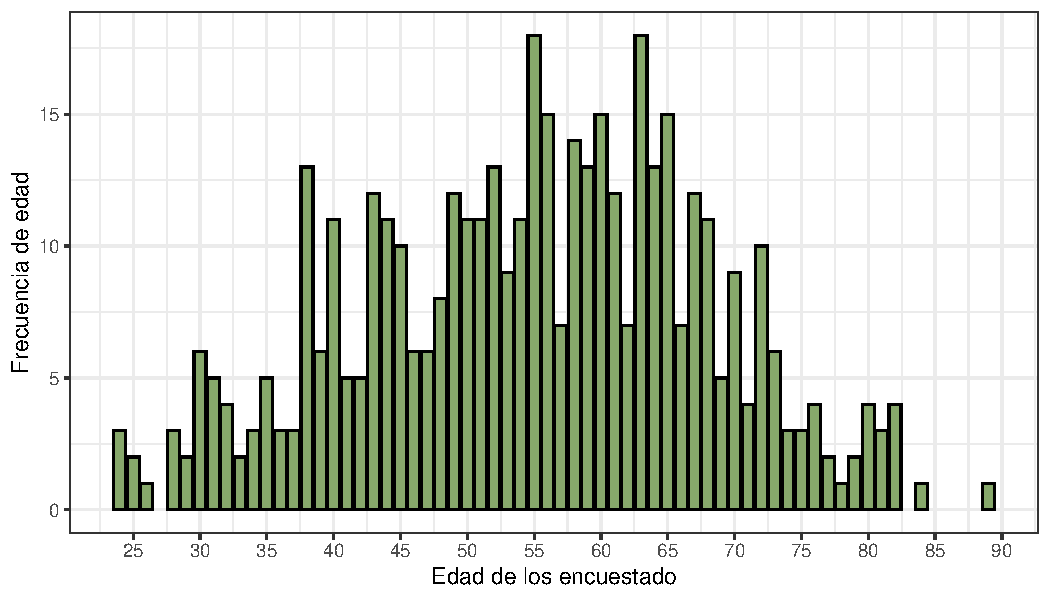
\includegraphics[width=\maxwidth]{figure/fig_uno-1} 
\end{knitrout}
  \caption*{Fuente: trabajo de campo}
\end{figure}
La Tabla que muestra las edades de los encuestados, revela que solo el 6.35\% de la muestra se encuentra en el rango de edad de (23.9, 33.3], lo que indica que hay una baja representación de jóvenes adultos, lo que podría sugerir que este grupo tiene un interés limitado, en el siguiente rango, de (33.3, 42.6], el porcentaje aumenta a 12.24\%, pero sigue siendo un grupo pequeño, lo que refuerza la idea de que los adultos jóvenes son poco representados en esta muestra a medida que se avanza hacia la mediana edad, en el rango de (42.6, 51.9], el porcentaje alcanza un 19.73\%, lo que refleja un aumento considerable en la representación de este grupo, el rango de (51.9, 61.1] tiene el mayor porcentaje, con un 28.80\%, lo que indica que la mayoría de los encuestados se encuentran en una etapa de vida más avanzada, lo que podría influir en sus respuestas debido a la mayor experiencia acumulada, en el rango de (61.1, 70.4], el 22.00\% también representa una proporción significativa, lo que refuerza la tendencia hacia una población de mayor edad, aportando una perspectiva más madura y reflexiva, en cuanto al rango de (70.4, 79.7], se observa que el 7.94\% de los encuestados pertenece a esta categoría, lo que sugiere que hay una presencia notable de personas mayores, mientras que el grupo de (79.7, 89.1] representa solo el 2.95\%, lo que indica que la muestra cuenta con pocos participantes en el rango de edad más avanzada esto podría influir en la comprensión de las necesidades de este grupo, dado su bajo nivel de representación. En conclusión, estos datos reflejan una población principalmente adulta y mayor, lo que implica que las opiniones y necesidades que se recogen en la encuesta están influenciadas por las experiencias y circunstancias propias de estos grupos etarios.

\begin{fotos}
{Aplicacion de encuestas}{1}
\end{fotos}


Se analizara el genero de los encuestados
\begin{table}[H]
  \centering
  \caption{Genero de los encuestados}

\begin{tabular}{lcl}
\toprule
\cellcolor[HTML]{87A96B}{\textcolor{black}{\textbf{GENERO}}} & \cellcolor[HTML]{87A96B}{\textcolor{black}{\textbf{Conteo}}} & \cellcolor[HTML]{87A96B}{\textcolor{black}{\textbf{Porcentaje}}}\\
\midrule
MUJER & 213 & 47.97\\
VARON & 231 & 52.03\\
\bottomrule
\end{tabular}

  \caption*{Fuente: Trabajo de campo}
\end{table}  

\begin{figure}[H]
  \centering
  \caption{Frecuencia del genero de los encuestados}
\begin{knitrout}
\definecolor{shadecolor}{rgb}{0.969, 0.969, 0.969}\color{fgcolor}
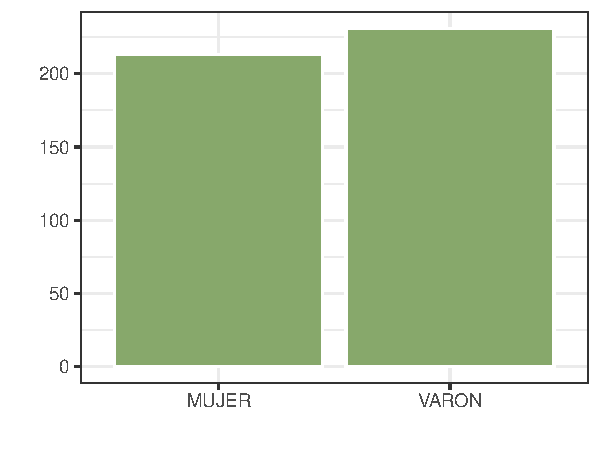
\includegraphics[width=\maxwidth]{figure/fig_dos-1} 
\end{knitrout}
  \caption*{Fuente: Trabajo de campo}
\end{figure}
La siguiente tabla  presenta la distribución de género entre los encuestados, donde el 47.97\% corresponde a mujeres y el 52.03\% a hombres, lo que refleja una ligera mayoría masculina en la muestra, aunque existe una ligera predominancia de varones, la representación femenina sigue siendo significativa y debe tenerse en cuenta al analizar los resultados, la diferencia de solo un 4.06\% entre ambos géneros sugiere que las experiencias y opiniones de los dos grupos están igualmente representadas, lo que podría aportar una diversidad de puntos de vista en las respuestas obtenidas. En conclusión, la distribución de género presentada en esta tabla muestra, una muestra equilibrada, aunque con una ligera inclinación hacia los varones, lo que es un aspecto importante a considerar en el análisis de los datos recopilados.
esta dispuesto a renuncio //



\begin{table}[H]
  \centering
  \caption{Grado de instruccion}

\begin{tabular}{lcl}
\toprule
\cellcolor[HTML]{87A96B}{\textcolor{black}{\textbf{Grado}}} & \cellcolor[HTML]{87A96B}{\textcolor{black}{\textbf{Conteo}}} & \cellcolor[HTML]{87A96B}{\textcolor{black}{\textbf{Porcentaje}}}\\
\midrule
NINGUNO & 95 & 22.73\\
PRIMARIA & 209 & 50.00\\
SECUNDARIA & 106 & 25.36\\
SUPERIOR & 5 & 1.20\\
TECNICO & 3 & 0.72\\
\bottomrule
\end{tabular}


  \caption*{Fuente: Trabajo de campo}
\end{table}
\begin{figure}[H]
  \centering
  \caption{Distribucion del grado de instruccion}
\begin{knitrout}
\definecolor{shadecolor}{rgb}{0.969, 0.969, 0.969}\color{fgcolor}
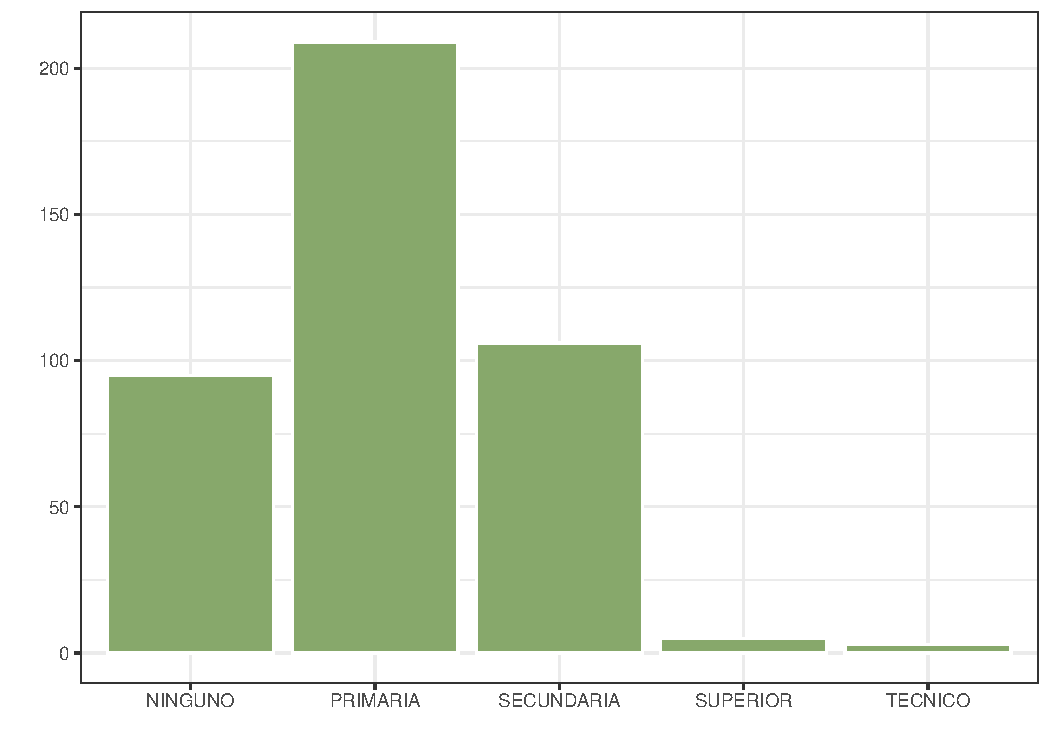
\includegraphics[width=\maxwidth]{figure/fig_tres-1} 
\end{knitrout}
  \caption*{Fuente: Trabajo de campo}
\end{figure}
la tabla muestra la distribución del grado de instrucción de los encuestados, donde se observa que el 50\% no ha completado la educación primaria, lo que indica una alta proporción de personas con bajo nivel educativo en la muestra. En comparación, el 22.73\% de los encuestados no tiene ningún grado de instrucción, lo que resalta la necesidad de atención a la educación en estas poblaciones encuestadas, el 25.36\% ha alcanzado la secundaria, lo que sugiere que una parte significativa ha completado al menos la educación básica, pero aún queda un porcentaje considerable que no ha avanzado más allá de este nivel, solo un 1.20\% ha alcanzado la educación superior, lo que indica que la mayoría de los encuestados no ha tenido acceso a la educación universitaria, lo que podría limitar sus oportunidades laborales y de desarrollo personal, por último, el 0.72\% ha completado estudios técnicos, lo que sugiere que la formación técnica también es escasa en esta población. En conclusión, estos porcentajes reflejan un panorama educativo preocupante, donde la mayoría de los encuestados tiene un bajo nivel de instrucción, lo que puede tener implicaciones significativas en su calidad de vida y en su capacidad para acceder a mejores oportunidades económicas y sociales.m modificando
\begin{fotos}
{Aplicacion de encuestas}{2}
\end{fotos}


\begin{table}[H]
  \centering
  \caption{Tipo de ingreso familiar}

\begin{tabular}{lcl}
\toprule
\cellcolor[HTML]{87A96B}{\textcolor{black}{\textbf{Ingreso}}} & \cellcolor[HTML]{87A96B}{\textcolor{black}{\textbf{Conteo}}} & \cellcolor[HTML]{87A96B}{\textcolor{black}{\textbf{Porcentaje}}}\\
\midrule
ANUAL & 240 & 61.22\\
MENSUAL & 126 & 32.14\\
QUINCENAL & 20 & 5.10\\
SEMANAL & 6 & 1.53\\
\bottomrule
\end{tabular}

  \caption*{Fuente: Trabajo de campo}
\end{table}

\begin{figure}[H]
  \centering
  \caption{Distribucion del tipo de ingreso familiar}
\begin{knitrout}
\definecolor{shadecolor}{rgb}{0.969, 0.969, 0.969}\color{fgcolor}
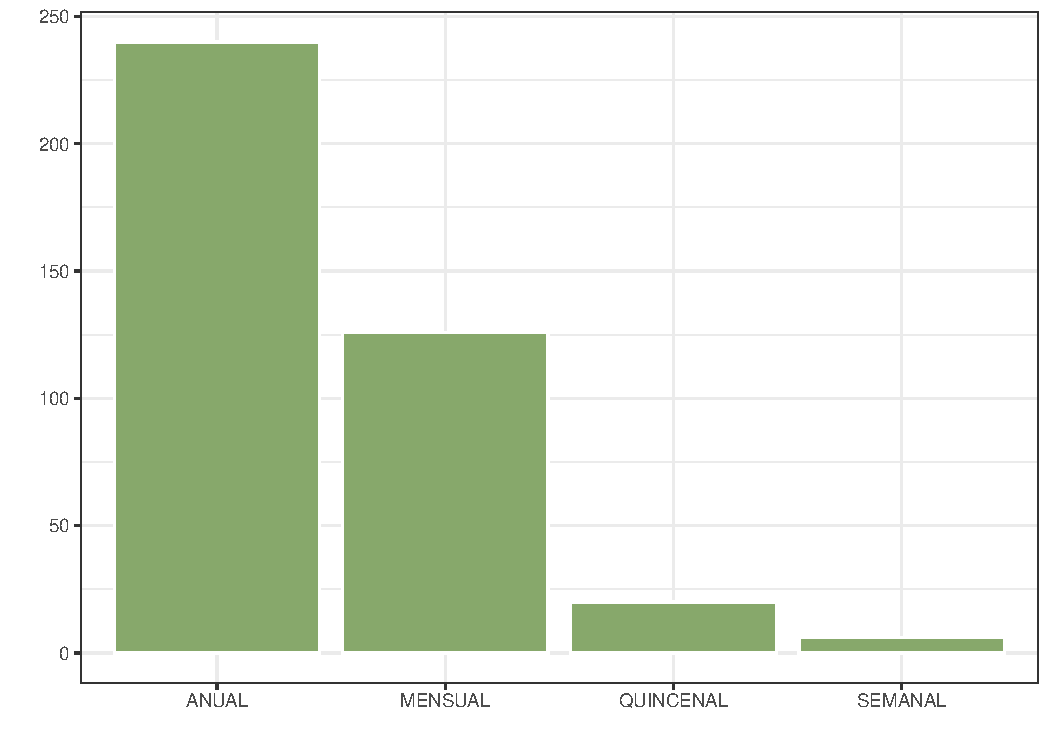
\includegraphics[width=\maxwidth]{figure/fig_cinco-1} 
\end{knitrout}
  \caption*{Fuente: Trabajo de campo}
\end{figure}
La tabla que presenta el tipo de ingreso familiar indica que el 61.22\% de los encuestados obtiene ingresos anuales, lo cual es especialmente relevante en el contexto agrícola, ya que muchos agricultores generan ingresos de forma estacional, dependiendo de las cosechas y de la comercialización de productos a lo largo del año, este patrón de ingresos anuales puede reflejar la naturaleza cíclica de la actividad agrícola, donde los ingresos son mayores durante las épocas de cosecha y tienden a disminuir en los períodos de inactividad, lo que podría generar dificultades en la planificación financiera y en la estabilidad económica de las familias del sector, en cambio, el 32.14\% de los encuestados que recibe ingresos mensuales podría estar asociado con aquellos que participan en actividades agrícolas más diversificadas o que tienen acceso a mercados más estables, lo que les permite contar con un flujo de ingresos más constante. Por otro lado, el 5.10\% de los encuestados que percibe ingresos quincenales y el 1.53\% que recibe ingresos semanales son proporciones reducidas, lo que sugiere que estos esquemas de pago son menos comunes en el sector agrícola, donde la mayoría de los ingresos provienen de pagos anuales o mensuales. En conjunto, estos datos reflejan la dependencia de las familias agrícolas en los ingresos anuales, lo que puede influir en su capacidad para gestionar los recursos y enfrentar la variabilidad inherente a la producción agrícola.
\begin{fotos}
{Aplicacion de encuestas}{3}
\end{fotos}


\begin{table}[H]
  \centering
  \caption{Ingreso familiar}

\begin{tabular}{lcl}
\toprule
\cellcolor[HTML]{87A96B}{\textcolor{black}{\textbf{Ingreso\_familiar}}} & \cellcolor[HTML]{87A96B}{\textcolor{black}{\textbf{Conteo}}} & \cellcolor[HTML]{87A96B}{\textcolor{black}{\textbf{Porcentaje}}}\\
\midrule
Mayor a S/1500 & 29 & 7.51\\
S/100 a S/500 & 269 & 69.69\\
S/501 a S/950 & 51 & 13.21\\
S/951 a S/1500 & 37 & 9.59\\
\bottomrule
\end{tabular}

  \caption*{Fuente: Trabajo de campo}
\end{table}


\begin{figure}[H]
  \centering
  \caption{Distribucion del tipo de ingreso familiar}
\begin{knitrout}
\definecolor{shadecolor}{rgb}{0.969, 0.969, 0.969}\color{fgcolor}
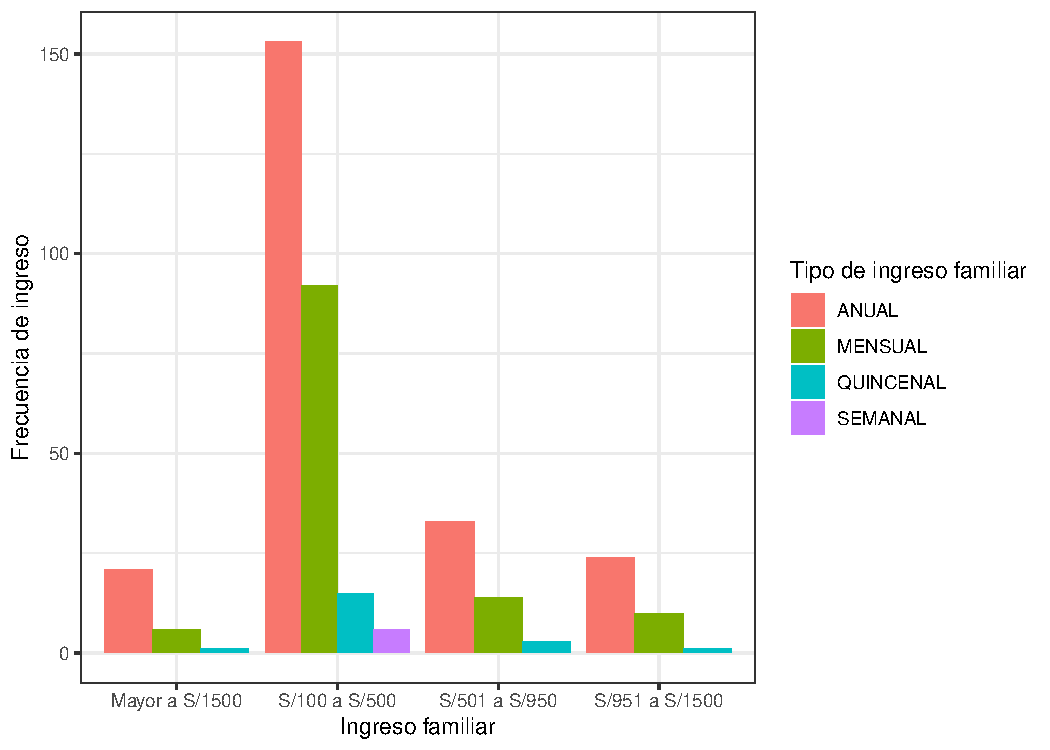
\includegraphics[width=\maxwidth]{figure/fig_seis-1} 
\end{knitrout}
  \caption*{Fuente: Trabajo de campo}
\end{figure}
Respecto a los ingresos familiares,la tabla indica que el 69.69\% de los encuestados reporta ingresos familiares que varían entre S/100 y S/500, lo que señala que una proporción considerable de la población se encuentra en una situación económica vulnerable, posiblemente reflejando los márgenes de ganancias reducidos de la producción agrícola, en la cual los costos de producción pueden superar los ingresos obtenidos, además, el 13.21\% de los encuestados indica que sus ingresos se encuentran entre S/501 y S/950, lo que sugiere que un grupo más pequeño de la población podría contar con ingresos relativamente más estables, aunque aún por debajo de una barrera que asegure un nivel adecuado de calidad de vida, solo el 7.51\% de los encuestados tiene ingresos superiores a S/1500, lo que denota que las familias con ingresos más altos son bastante escasas, lo que podría reflejar las dificultades de los agricultores para acceder a mercados más rentables o la falta de diversificación en sus fuentes de ingreso, finalmente, el 9.59\% de los encuestados que percibe entre S/951 y S/1500 también representa un porcentaje bajo, lo que refuerza la idea de que la mayoría de las familias agrícolas enfrenta serias limitaciones económicas. En resumen, estos datos sugieren que la producción agrícola en esta población está asociada con ingresos bajos y una alta vulnerabilidad económica, lo que podría impactar negativamente su capacidad para invertir en mejoras productivas y en el bienestar de sus hogares
\begin{fotos}
{Sensibililzacion a los beneficiarios}{4}
\end{fotos}


\begin{table}[H]
  \centering
  \caption{Numero de integrantes que conforman su familia}

\begin{tabular}{lcl}
\toprule
\cellcolor[HTML]{87A96B}{\textcolor{black}{\textbf{Integrantes}}} & \cellcolor[HTML]{87A96B}{\textcolor{black}{\textbf{Conteo}}} & \cellcolor[HTML]{87A96B}{\textcolor{black}{\textbf{Porcentaje}}}\\
\midrule
3 A 5 PERSONAS & 228 & 51.35\\
MAS DE 6 PERSONAS & 41 & 9.23\\
MENOS DE 2 PERSONAS & 175 & 39.41\\
\bottomrule
\end{tabular}


  \caption*{Fuente: Trabajo de campo}
\end{table}

\begin{figure}[H]
  \centering
  \caption{Numero de integrantes que conforman su familia}
\begin{knitrout}
\definecolor{shadecolor}{rgb}{0.969, 0.969, 0.969}\color{fgcolor}
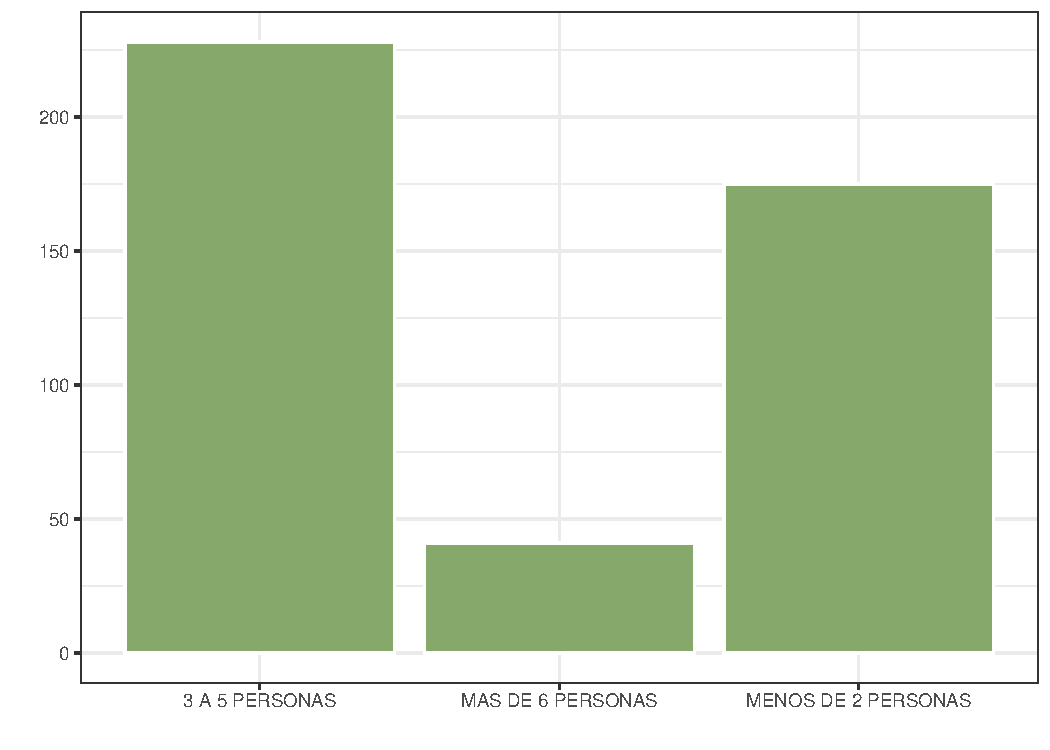
\includegraphics[width=\maxwidth]{figure/fig_siete-1} 
\end{knitrout}
  \caption*{Fuente: Trabajo de campo}
\end{figure}
En cuanto al número de miembros que componen las familias, se observa que el 51.35\% de los encuestados tiene entre 3 y 5 personas en su hogar, lo que indica que la mayoría de las familias son de tamaño moderado, esto podría ser característico de las comunidades agrícolas, donde las familias suelen ser más pequeñas para facilitar la gestión de los recursos y la participación en las actividades productivas además, el 39.41\% de las familias cuenta con más de 6 integrantes, lo que sugiere que una proporción considerable de la población vive en hogares más grandes, esto podría conllevar una mayor carga económica, lo que haría necesario que más miembros de la familia contribuyan tanto a la producción agrícola como a otras fuentes de ingreso, lo que a su vez podría generar presión sobre los recursos disponibles, por otro lado, el 9.23\% de las familias tiene menos de 2 miembros, un porcentaje relativamente bajo, lo que podría reflejar situaciones de hogares unipersonales, que son menos frecuentes en contextos agrícolas donde la mano de obra familiar es esencial para las actividades productivas. En resumen, estos datos sugieren que la estructura familiar en esta población está influenciada por la dinámica de la producción agrícola, donde el tamaño de la familia puede tener un impacto directo tanto en la capacidad laboral como en la distribución de los recursos económicos.
\begin{fotos}
{Aplicacion de encuestas en el area de influencia}{5}
\end{fotos}


\begin{table}[H]
  \centering
  \caption{Actividad economica a la que se dedica}

\begin{tabular}{lcl}
\toprule
\cellcolor[HTML]{87A96B}{\textcolor{black}{\textbf{Actividad}}} & \cellcolor[HTML]{87A96B}{\textcolor{black}{\textbf{Conteo}}} & \cellcolor[HTML]{87A96B}{\textcolor{black}{\textbf{Porcentaje}}}\\
\midrule
AGRICULTOR & 146 & 32.74\\
AGROPECUARIO & 156 & 34.98\\
AMA DE CASA & 126 & 28.25\\
COMERCIANTE & 6 & 1.35\\
PECUARIO & 8 & 1.79\\
\addlinespace
TRABAJADOR PUBLICO & 4 & 0.90\\
\bottomrule
\end{tabular}

  \caption*{Fuente: Trabajo de campo}
\end{table}

\begin{figure}[H]
  \centering
  \caption{Actividad economica a la que se dedica}
\begin{knitrout}
\definecolor{shadecolor}{rgb}{0.969, 0.969, 0.969}\color{fgcolor}
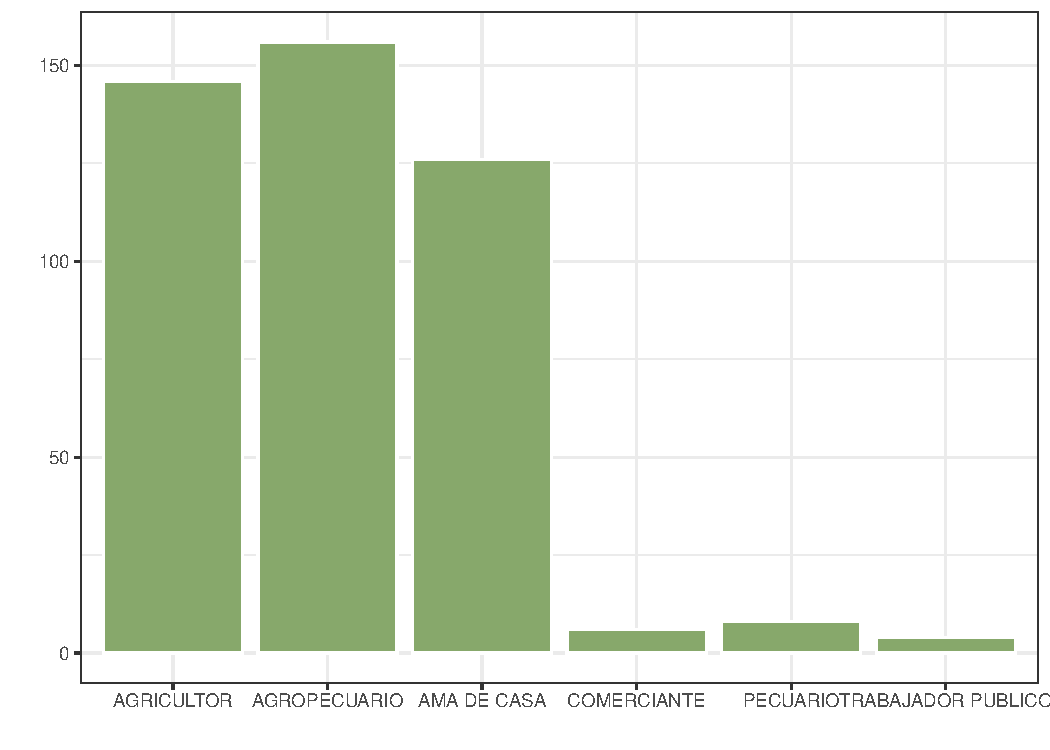
\includegraphics[width=\maxwidth]{figure/fig_ocho-1} 
\end{knitrout}
  \caption*{Fuente: Trabajo de campo}
\end{figure}
La tabla que muestra la actividad económica de los usuarios encuestados revela que el 34.98\% se dedica a actividades agropecuarias, lo que indica que una proporción considerable de la población está involucrada en la producción tanto agrícola como ganadera, subrayando la relevancia de estas actividades en la economía local, además el 32.74\% de los usuarios encuestados se dedica a la agricultura, lo que sugiere que la mayoría está comprometida con la siembra de cultivos, lo cual puede ser un indicio de la dependencia de la comunidad de la agricultura como fuente primaria de ingresos y sustento, por otro lado el 28.25\% se identifica como ama de casa, lo que podría indicar que muchas mujeres en las comunidades están encargadas de las tareas domésticas, aunque también es posible que estén involucradas en actividades agrícolas de manera informal, solo el 1.35\% se dedica al comercio y el 0.90\% al trabajo en el sector público, lo que refleja que las oportunidades laborales fuera del ámbito agrícola son limitadas. En conclusión, estos datos muestran una marcada orientación hacia la producción agrícola en las comunidades encuestadas, lo cual puede tener importantes implicaciones en términos de desarrollo económico, seguridad alimentaria y estabilidad de los ingresos familiares.
\begin{fotos}
{Aplicacion de encuestas en el area de influencia}{6}
\end{fotos}


\begin{table}[H]
  \centering
  \caption{Cuenta con el servicio de agua potable}

\begin{tabular}{lcl}
\toprule
\cellcolor[HTML]{87A96B}{\textcolor{black}{\textbf{Agua}}} & \cellcolor[HTML]{87A96B}{\textcolor{black}{\textbf{Conteo}}} & \cellcolor[HTML]{87A96B}{\textcolor{black}{\textbf{Porcentaje}}}\\
\midrule
NO & 3 & 0.67\\
SI & 445 & 99.33\\
\bottomrule
\end{tabular}

  \caption*{Fuente: Trabajo de campo}
\end{table}

\begin{figure}[H]
  \centering
  \caption{Cuenta con el servicio de agua potable}
\begin{knitrout}
\definecolor{shadecolor}{rgb}{0.969, 0.969, 0.969}\color{fgcolor}
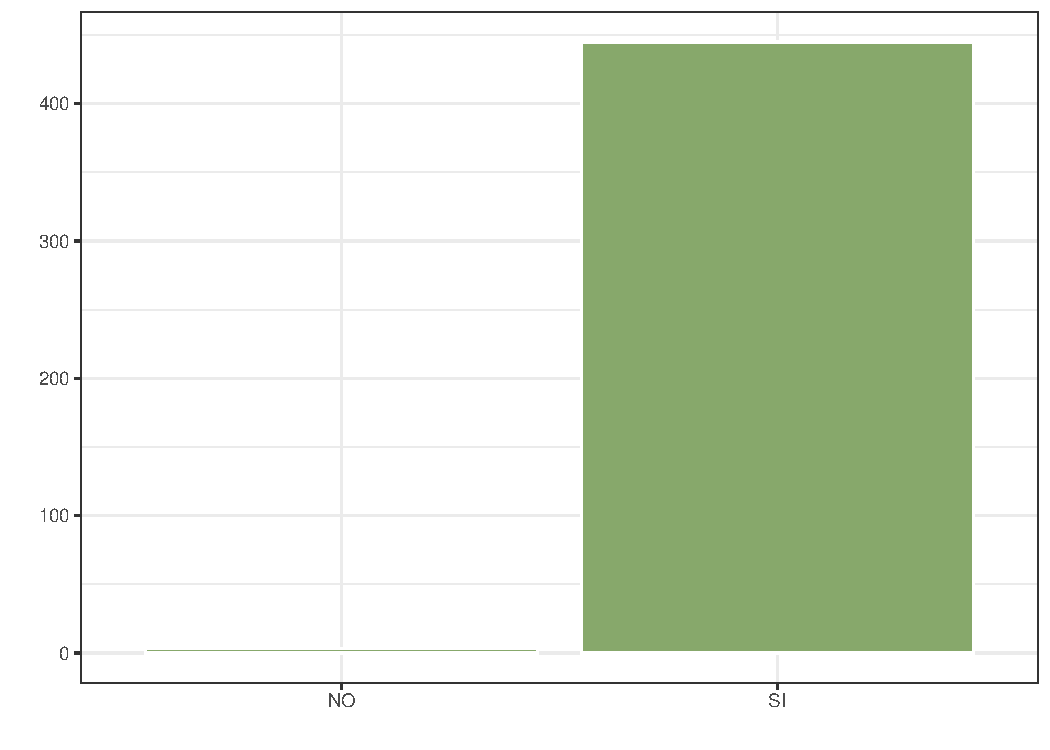
\includegraphics[width=\maxwidth]{figure/fig_nueve-1} 
\end{knitrout}
  \caption*{Fuente: Trabajo de campo}
\end{figure}
Respecto al servicio de agua potable indica que el 99.33\% de los usuarios encuestados cuenta con este servicio, este alto porcentaje sugiere que la infraestructura de agua potable en las  comunidades encuestadas es efectiva, lo que puede contribuir a mejorar la calidad de vida y reducir enfermedades relacionadas con el agua contaminada, sin embargo el 0.67\% que no tiene acceso a este servicio representa una preocupación, ya que podría enfrentar riesgos significativos para la salud y dificultades en la realización de actividades diarias, lo que resalta la necesidad de seguir trabajando en la cobertura y calidad del suministro de agua para garantizar que todos los miembros de las comunidades tengan acceso a este recurso vital.
\begin{fotos}
{Aplicacion de encuestas en el area de influencia}{7}
\end{fotos}


\begin{table}[H]
  \centering
  \caption{Tipo de agua que consume}

\begin{tabular}{lcl}
\toprule
\cellcolor[HTML]{87A96B}{\textcolor{black}{\textbf{Agua\_que\_consume}}} & \cellcolor[HTML]{87A96B}{\textcolor{black}{\textbf{Conteo}}} & \cellcolor[HTML]{87A96B}{\textcolor{black}{\textbf{Porcentaje}}}\\
\midrule
CLORADA & 327 & 75.00\\
POTABLE & 91 & 20.87\\
SIN TRATAR & 18 & 4.13\\
\bottomrule
\end{tabular}

  \caption*{Fuente: Trabajo de campo}
\end{table}

\begin{figure}[H]
  \centering
  \caption{Tipo de agua que consume}
\begin{knitrout}
\definecolor{shadecolor}{rgb}{0.969, 0.969, 0.969}\color{fgcolor}
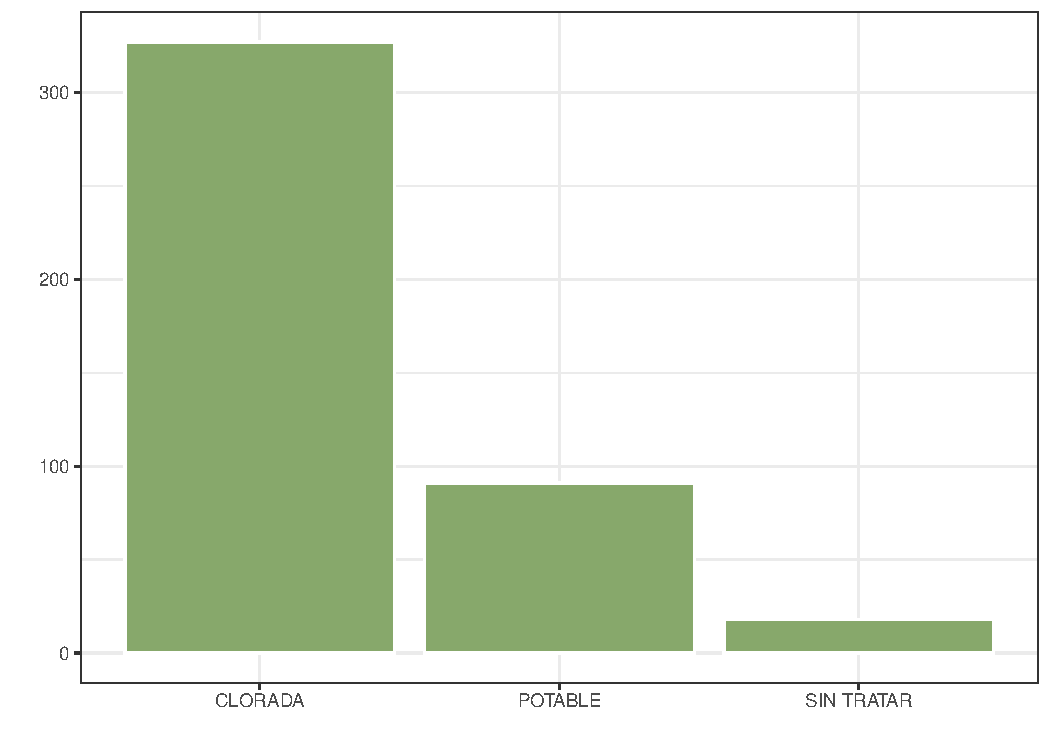
\includegraphics[width=\maxwidth]{figure/fig_diez-1} 
\end{knitrout}
  \caption*{Fuente: Trabajo de campo}
\end{figure}
La siguiente tabla muestra el tipo de agua consumida por la población, un 75\% de los encuestados utiliza agua clorada, lo que indica que la mayoría de las personas opta por una fuente tratada, lo que proporciona una mayor garantía de calidad y seguridad en el consumo, lo cual es importante  para la salud pública, por otro lado el 20.87\% consume agua potable, lo que sugiere que una porción de la población tiene acceso a agua que, aunque no ha sido tratada, se considera apta para el consumo humano, esto podría reflejar una dependencia de fuentes naturales o locales de abastecimiento, sin embargo el 4.13\% que utiliza agua sin tratar representa un segmento vulnerable que podría estar expuesto a riesgos sanitarios, como la contaminación microbiológica o química que es dañino para la salud, por ello es importante continuar fortaleciendo la infraestructura de abastecimiento de agua, así como las campañas de educación sobre prácticas de consumo seguro, para garantizar que toda la comunidad cuente con acceso a agua potable de calidad, protegiendo así la salud pública y contribuyendo al bienestar general.
\begin{fotos}
{sensibilizacion a la poblacion}{8}
\end{fotos}




\begin{table}[H]
  \centering
  \caption{Fuente de agua}

\begin{tabular}{lcl}
\toprule
\cellcolor[HTML]{87A96B}{\textcolor{black}{\textbf{Abastecimiento\_agua}}} & \cellcolor[HTML]{87A96B}{\textcolor{black}{\textbf{Conteo}}} & \cellcolor[HTML]{87A96B}{\textcolor{black}{\textbf{Porcentaje}}}\\
\midrule
MANTIAL & 323 & 72.91\\
PILON DE USO PUBLICO & 13 & 2.93\\
RED PUBLICA & 94 & 21.22\\
RIO O RIACHUELO & 13 & 2.93\\
\bottomrule
\end{tabular}

  \caption*{Fuente: Trabajo de campo}
\end{table}

\begin{figure}[H]
  \centering
  \caption{Fuente de agua}
\begin{knitrout}
\definecolor{shadecolor}{rgb}{0.969, 0.969, 0.969}\color{fgcolor}
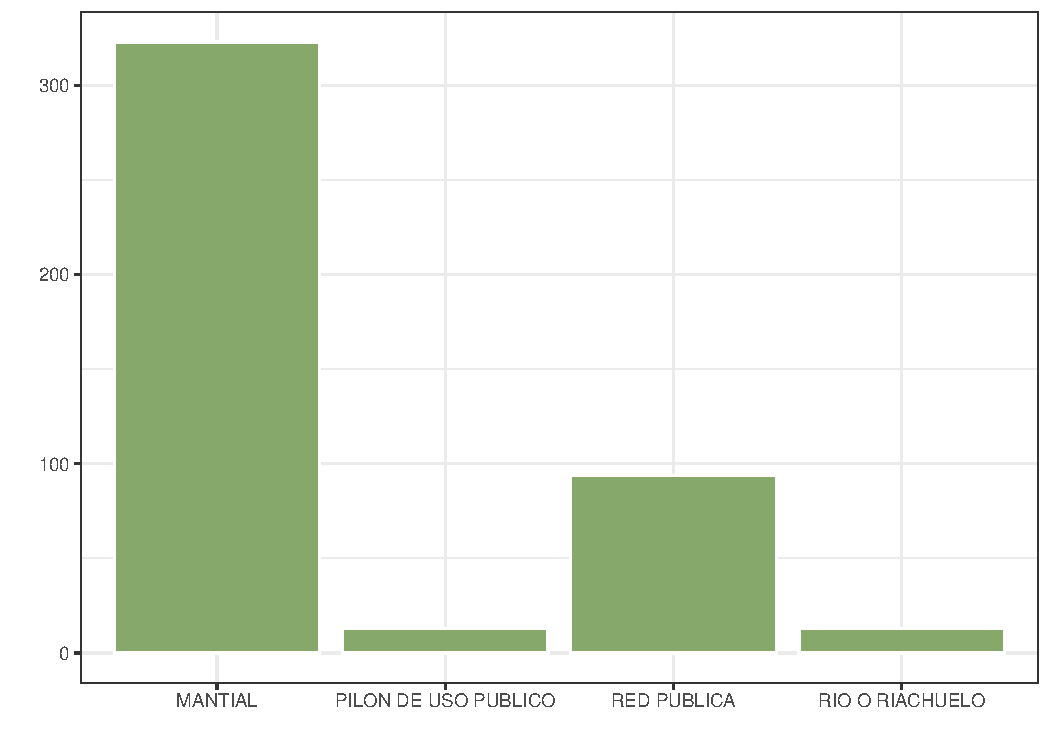
\includegraphics[width=\maxwidth]{figure/fig_once-1} 
\end{knitrout}
  \caption*{Fuente: Trabajo de campo}
\end{figure}
En la siguiente tabla se detalla las fuentes de agua utilizadas por la población indica  que el 72.91\% de los encuestados obtiene el agua de un manantial, lo que refleja una considerable dependencia de este recurso natural, sugiriendo que las fuentes de agua en las comunidades son esenciales para el abastecimiento diario del recurso, este dato resalta la importancia de contar con una infraestructura adecuada que permita la captación y distribución de agua proveniente de manantiales, los cuales suelen ser una fuente confiable y natural de agua, aunque también pueden estar sujetos a variaciones estacionales o contaminaciones si no se gestionan adecuadamente, por otro lado el 21.22\% de la población accede al agua a través de una red pública, lo que pone de manifiesto la importancia de los sistemas públicos de abastecimiento en las comunidades, el 2.93\% de los encuestados obtiene agua de un pilón de uso público, mientras que otro 2.93\% lo hace de un río o riachuelo. Estos datos reflejan que una pequeña porción de la población depende de fuentes de agua menos controladas y tratadas. Para reducir los riesgos sanitarios y promover un acceso equitativo al agua potable, sería necesario fortalecer la infraestructura de distribución pública, así como implementar medidas de control de calidad más estrictas en las fuentes naturales y comunitarias. De esta manera, se contribuiría a la salud pública y se mejoraría la calidad de vida de las comunidades en su conjunto.
\begin{fotos}
{sensibilizacion a la poblacion}{9}
\end{fotos}

\begin{table}[H]
  \centering
  \caption{Energia electrica}

\begin{tabular}{lcl}
\toprule
\cellcolor[HTML]{87A96B}{\textcolor{black}{\textbf{Electricidad}}} & \cellcolor[HTML]{87A96B}{\textcolor{black}{\textbf{Conteo}}} & \cellcolor[HTML]{87A96B}{\textcolor{black}{\textbf{Porcentaje}}}\\
\midrule
NO & 26 & 5.83\\
SI & 420 & 94.17\\
\bottomrule
\end{tabular}

  \caption*{Fuente: Trabajo de campo}
\end{table}

\begin{figure}[H]
  \centering
  \caption{Energia electrica}
\begin{knitrout}
\definecolor{shadecolor}{rgb}{0.969, 0.969, 0.969}\color{fgcolor}
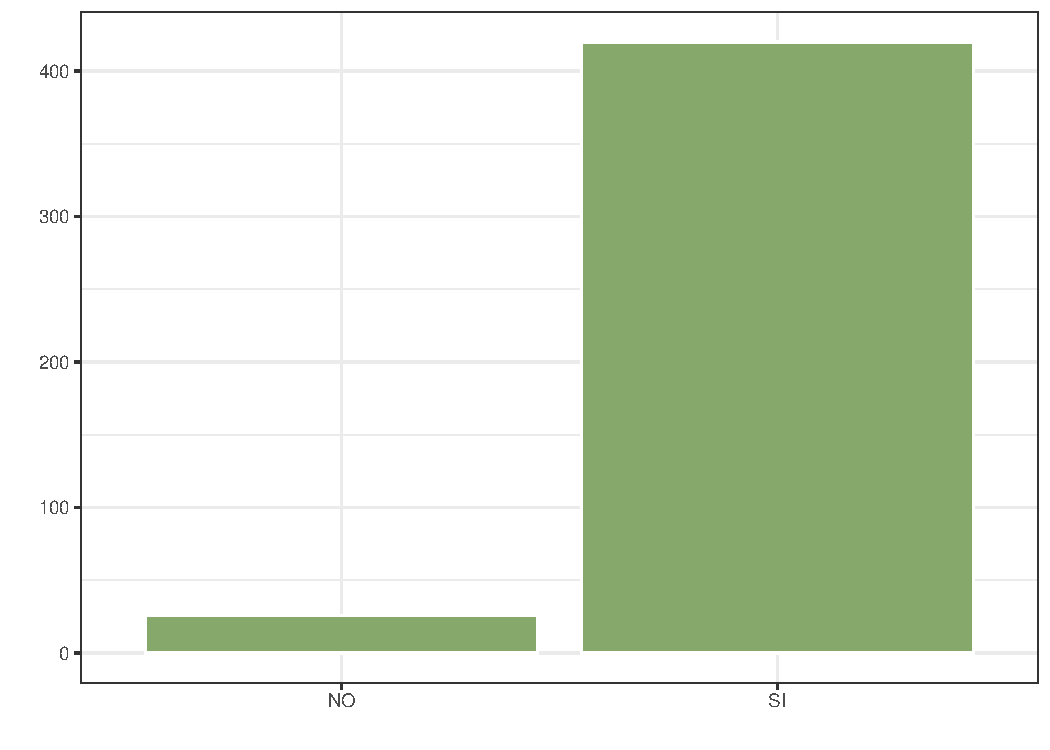
\includegraphics[width=\maxwidth]{figure/fig_doce-1} 
\end{knitrout}
  \caption*{Fuente: Trabajo de campo}
\end{figure}
Respecto el acceso a la energía eléctrica muestra que un 94.17\% de los encuestados dispone de este servicio, lo que demuestra que la gran mayoría de la población tiene acceso a una fuente de energía vital para llevar a cabo actividades diarias, realizar labores agrícolas y mantener el funcionamiento de negocios, este alto porcentaje refleja un importante avance en la cobertura de energía eléctrica, lo que facilita el progreso económico y social en las comunidades, al proporcionar la base para el desarrollo de diversas actividades productivas y el acceso a tecnologías de información, por otro lado el 5.83\% que no tiene acceso a la energía eléctrica, la falta de acceso a este servicio esencial puede generar obstáculos significativos para su calidad de vida, afectando su capacidad para realizar tareas cotidianas, acceder a servicios educativos, sanitarios o de comunicación, e incluso mejorar sus condiciones laborales. Es fundamental seguir trabajando en la expansión de la infraestructura energética y en la implementación de políticas públicas que aseguren que el acceso a la energía eléctrica sea para todos, para así fomentar una mayor equidad y mejorar las condiciones de vida de toda la población.
\begin{fotos}
{sensibilizacion a la poblacion}{10}
\end{fotos}

\begin{comment}
\begin{table}[H]
  \centering
  \caption{Energia electrica}

  \caption*{Fuente: Trabajo de campo}
\end{table}

\begin{figure}[H]
  \centering
  \caption{Energia electrica}

  \caption*{Fuente: Trabajo de campo}
\end{figure}


%\begin{fotos}
%{sensibilizacion a la poblacion}{11}
%\end{fotos}
\end{comment}

\begin{table}[H]
  \centering
  \caption{Persona que trabaja en la parcela}

\begin{tabular}{lcl}
\toprule
\cellcolor[HTML]{87A96B}{\textcolor{black}{\textbf{Trabaja}}} & \cellcolor[HTML]{87A96B}{\textcolor{black}{\textbf{Conteo}}} & \cellcolor[HTML]{87A96B}{\textcolor{black}{\textbf{Porcentaje}}}\\
\midrule
OTRO & 4 & 0.89\\
UN AMIGO & 5 & 1.12\\
UN FAMILIAR & 35 & 7.83\\
USTED MISMO & 403 & 90.16\\
\bottomrule
\end{tabular}

  \caption*{Fuente: Trabajo de campo}
\end{table}

\begin{figure}[H]
  \centering
  \caption{Persona que trabaja en la parcela}
\begin{knitrout}
\definecolor{shadecolor}{rgb}{0.969, 0.969, 0.969}\color{fgcolor}
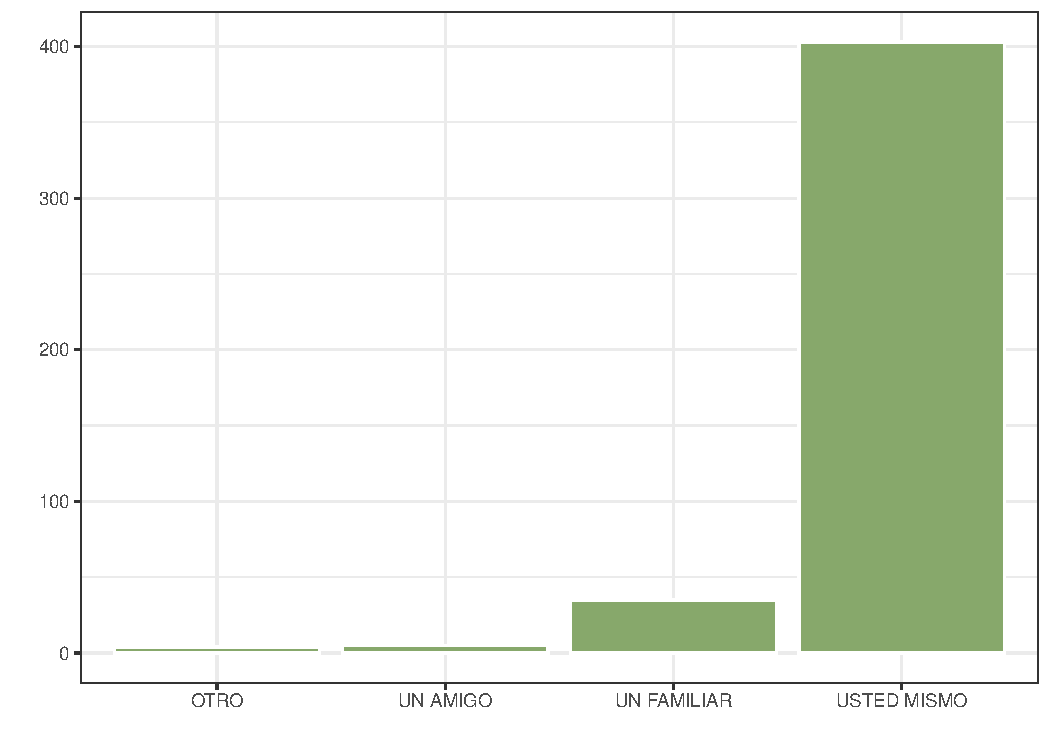
\includegraphics[width=\maxwidth]{figure/fig_catorce-1} 
\end{knitrout}
  \caption*{Fuente: Trabajo de campo}
\end{figure}
Respecto a quien realiza las actividades de campo en la parcela destinada al cultivo, mediante la encuesta podemos detallar lo siguiente, el 90,16\% de los usuarios realiza sus propias actividades durante la siembra y cosecha, el 7,83\% de los agricultores realiza las actividades agrícolas o está a responsabilidad de un familiar,un 1,12\% de los productores agricoles esta a responsabilidad de un amigo y el 0.89\% prefiere que otra persona se lo haga el cultivo por lo tanto, se concluye que los usuarios del comité de agua prefieren ellos mismos hacer sus actividades agricolas, podemos apreciar la tabla y grafico:
\begin{fotos}
{sensibilizacion a la poblacion}{12}
\end{fotos}


\begin{tablas}
{uso de la parcela en el ultimo año}{

\begin{tabular}{lcl}
\toprule
\cellcolor[HTML]{87A96B}{\textcolor{black}{\textbf{Uso\_parcela}}} & \cellcolor[HTML]{87A96B}{\textcolor{black}{\textbf{Conteo}}} & \cellcolor[HTML]{87A96B}{\textcolor{black}{\textbf{Porcentaje}}}\\
\midrule
CULTIVOS PERMANENTES & 252 & 57.27\\
CULTIVOS TRANSITORIOS & 165 & 37.50\\
PASTOS NATURALES & 23 & 5.23\\
\bottomrule
\end{tabular}

}
\end{tablas}

\begin{graficas}
{uso de la parcela en el ultimo año}{
\begin{knitrout}
\definecolor{shadecolor}{rgb}{0.969, 0.969, 0.969}\color{fgcolor}
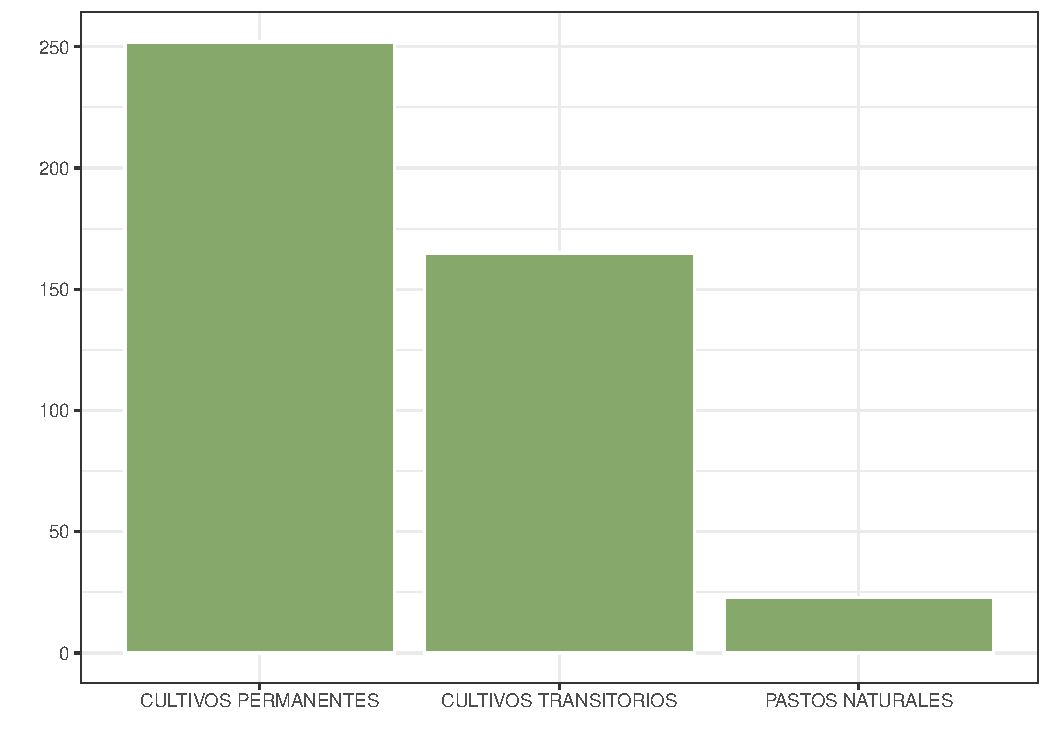
\includegraphics[width=\maxwidth]{figure/fig_quince-1} 
\end{knitrout}

}
\end{graficas}
La tabla  revela que el 57.27\% de las parcelas se utiliza para cultivos permanentes, lo que sugiere que los agricultores están invirtiendo en prácticas agrícolas sostenibles y buscando estabilidad en su producción a largo plazo, este enfoque puede resultar en una mayor productividad y seguridad alimentaria, ya que los cultivos permanentes suelen ser más resistentes a las fluctuaciones del mercado, en comparación con, el 37.50\% de las parcelas se dedica a cultivos transitorios, lo que indica que los agricultores también están adoptando una estrategia de diversificación, permitiéndoles adaptarse a las demandas del mercado y maximizar sus ingresos en el corto plazo, sin embargo el bajo porcentaje de 5.23\% destinado a pastos naturales sugiere que la producción ganadera no es una prioridad en esta área, lo que podría limitar las oportunidades de diversificación de ingresos de los agricultores, ya que depender únicamente de cultivos puede hacerlos más vulnerables a cambios en el clima o en el mercado. En conclusión, aunque la combinación de cultivos permanentes y transitorios puede ofrecer un enfoque equilibrado hacia la productividad agrícola, la falta de atención a los pastos naturales podría ser un área de mejora para aumentar la rentabilidad y la sostenibilidad a largo plazo.
\begin{fotos}
{sensibilizacion a la poblacion}{13}
\end{fotos}



\begin{tablas}
{Modalidad de tenencia de la parcela}{

\begin{tabular}{lcl}
\toprule
\cellcolor[HTML]{87A96B}{\textcolor{black}{\textbf{tenencia}}} & \cellcolor[HTML]{87A96B}{\textcolor{black}{\textbf{Conteo}}} & \cellcolor[HTML]{87A96B}{\textcolor{black}{\textbf{Porcentaje}}}\\
\midrule
ALQUILER & 1 & 0.22\\
OTRO & 8 & 1.78\\
PRESTADO O CEDIDO & 1 & 0.22\\
PROPIA & 242 & 53.90\\
TIERRAS COMUNALES & 197 & 43.88\\
\bottomrule
\end{tabular}

}
\end{tablas}

\begin{graficas}
{Modalidad de tenencia de la parcela}{
\begin{knitrout}
\definecolor{shadecolor}{rgb}{0.969, 0.969, 0.969}\color{fgcolor}
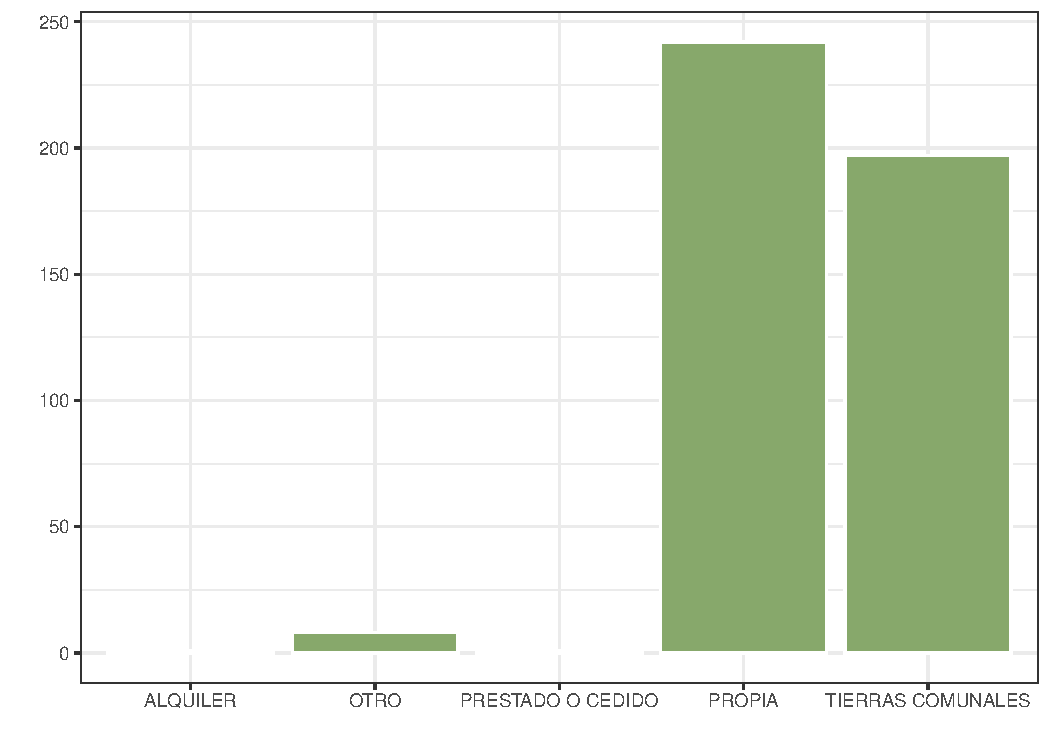
\includegraphics[width=\maxwidth]{figure/fig_dieciseis-1} 
\end{knitrout}
}
\end{graficas}

La Tabla muestra que el 53.90\% de las parcelas son de tenencia propia, lo que indica que la mayoría de los agricultores tienen un control directo sobre sus tierras, lo que puede fomentar una mayor inversión en prácticas agrícolas sostenibles y a largo plazo, ya que los propietarios suelen estar más motivados para mejorar la productividad de sus parcelas, por el contrario el 43.88\% de las parcelas son tierras comunales, lo que sugiere que una parte significativa de la producción agrícola depende de recursos compartidos, lo que podría limitar la capacidad de los agricultores para implementar mejoras individuales y optimizar la productividad, ademas el 1.78\% de las parcelas se encuentra en alquiler y el 0.22\% en prestado o cedido, lo que indica que la tenencia temporal puede ser menos común, pero también puede llevar a una menor inversión en la tierra, ya que los arrendatarios pueden no tener el mismo incentivo para mejorar la productividad a largo plazo. En conclusión, la predominancia de la tenencia propia sugiere un potencial significativo para la productividad agrícola, pero la dependencia de tierras comunales podría presentar desafíos en la implementación de prácticas agrícolas más eficientes y sostenibles.
\begin{fotos}
{aplicacion de encuestas}{14}
\end{fotos}


\begin{tablas}
{Tipo de documento de la parcela}{

\begin{tabular}{lcl}
\toprule
\cellcolor[HTML]{87A96B}{\textcolor{black}{\textbf{Documento\_parcela}}} & \cellcolor[HTML]{87A96B}{\textcolor{black}{\textbf{Conteo}}} & \cellcolor[HTML]{87A96B}{\textcolor{black}{\textbf{Porcentaje}}}\\
\midrule
HERENCIA & 41 & 9.19\\
OTRO & 31 & 6.95\\
POSESIONARIO & 139 & 31.17\\
TITULO COMUNAL & 200 & 44.84\\
TITULO PROPIO & 35 & 7.85\\
\bottomrule
\end{tabular}

}
\end{tablas}

\begin{graficas}
{Tipo de documento de la parcela}{
\begin{knitrout}
\definecolor{shadecolor}{rgb}{0.969, 0.969, 0.969}\color{fgcolor}
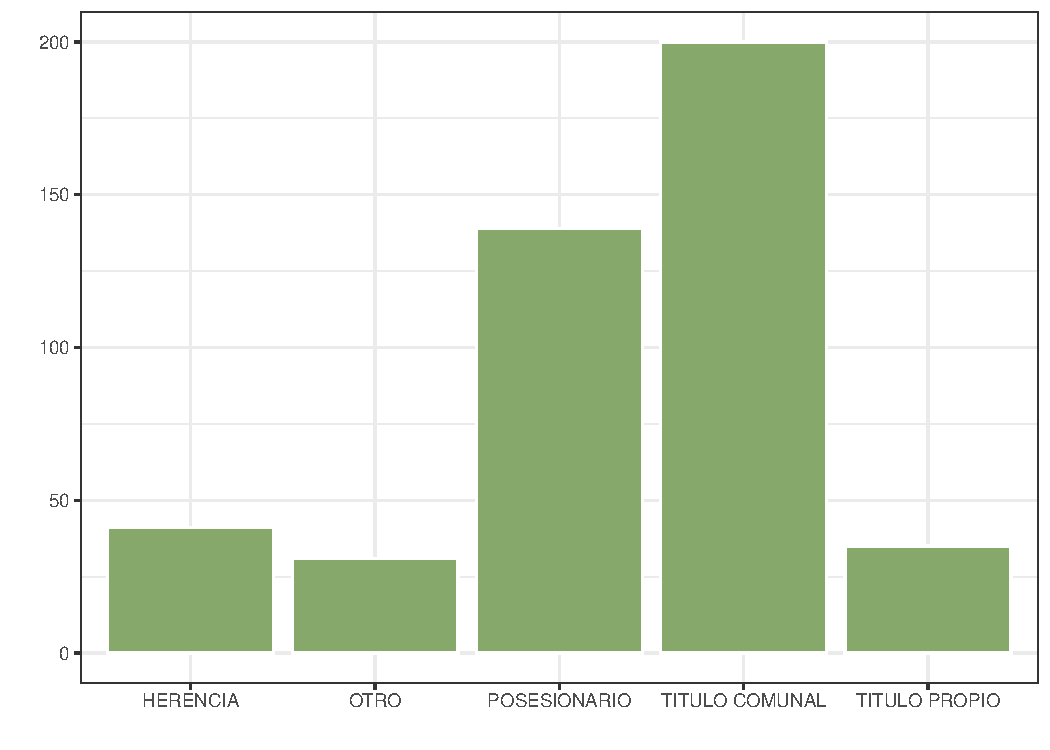
\includegraphics[width=\maxwidth]{figure/fig_diesiete-1} 
\end{knitrout}
}
\end{graficas}
La siguiente tabla indica que el 44.84\% de las parcelas cuenta con títulos comunales, lo que sugiere que una parte considerable de los agricultores tiene un reconocimiento formal de su propiedad, lo que puede facilitar el acceso a créditos y recursos para mejorar la productividad agrícola, un 7,85\% de los usuarios encuestados cuenta con un título propio, por otro lado el 31.17\% de las parcelas se clasifica como posesionario, lo que implica que estos agricultores pueden no tener un título formal, lo que podría limitar su capacidad para invertir en mejoras a largo plazo y acceder a financiamiento, afectando así su productividad además, el 9.19\% de las parcelas se destina a herencia y el 6.95\% a otros tipos de documentos, lo que sugiere que una porción menor de la población agrícola puede estar lidiando con incertidumbres legales sobre la tenencia de la tierra, lo que podría impactar negativamente en su motivación para invertir en la productividad. En conclusión, la predominancia de títulos comunales es un factor positivo para la productividad agrícola, mientras que la alta proporción de parcelas sin títulos formales puede representar un obstáculo significativo para el desarrollo y la mejora de las prácticas agrícolas en la región.
\begin{fotos}
{reconocimiento en campo}{15}
\end{fotos}


\begin{tablas}
{Organizacion a la que pertenece}{

\begin{tabular}{lcl}
\toprule
\cellcolor[HTML]{87A96B}{\textcolor{black}{\textbf{Tipo\_organizacion}}} & \cellcolor[HTML]{87A96B}{\textcolor{black}{\textbf{Conteo}}} & \cellcolor[HTML]{87A96B}{\textcolor{black}{\textbf{Porcentaje}}}\\
\midrule
COMISION DE REGANTES & 201 & 45.48\\
COMITE DE USUARIOS & 171 & 38.69\\
JUNTA DE USUARIOS & 70 & 15.84\\
\bottomrule
\end{tabular}


}
\end{tablas}

\begin{graficas}
{Organizacion a la que pertenece}{
\begin{knitrout}
\definecolor{shadecolor}{rgb}{0.969, 0.969, 0.969}\color{fgcolor}
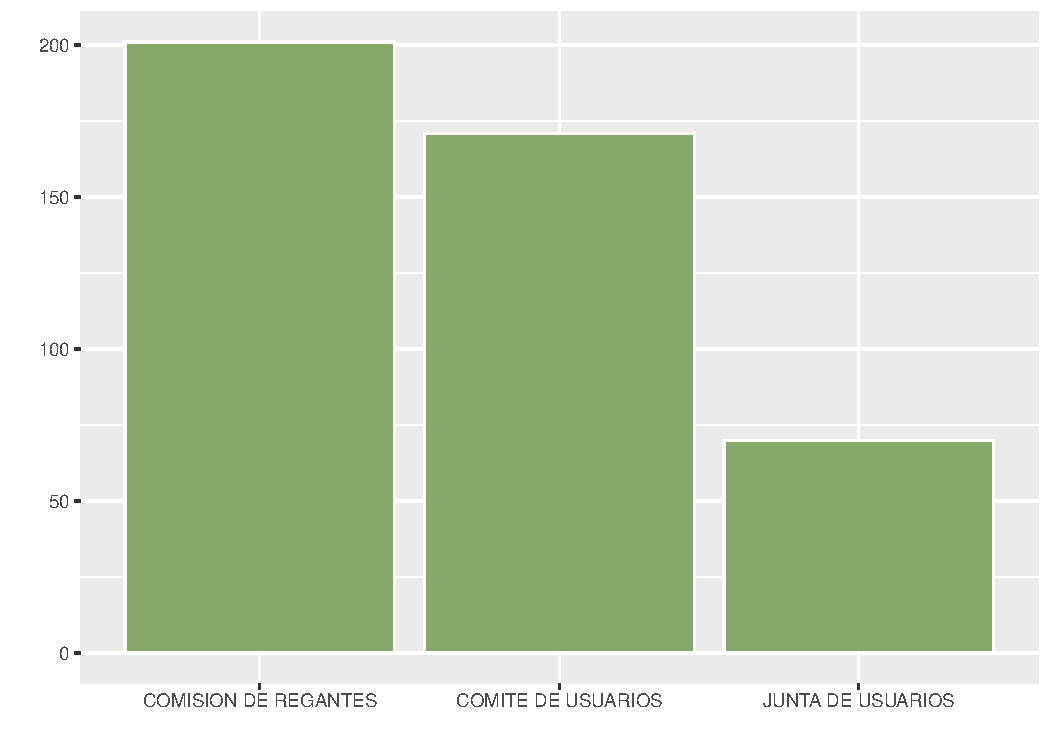
\includegraphics[width=\maxwidth]{figure/fig_dieciocho-1} 
\end{knitrout}
}
\end{graficas}
La tabla muestra que el 45.48\% de los agricultores está asociado a una Comisión de Regantes, lo que refleja una fuerte organización en torno a la gestión del agua, un recurso clave para la producción agrícola, esto sugiere que estos agricultores están comprometidos con la cooperación para optimizar el uso del agua en sus cultivos, además el 38.69\% está vinculado a un Comité de Usuarios, lo que refuerza la idea de que la colaboración y la organización son esenciales para enfrentar desafíos comunes y mejorar la eficiencia en la producción, por otro lado el 15.84\% que forma parte de una Junta de Usuarios indica que, aunque existe una participación considerable en estas organizaciones, todavía hay un porcentaje importante de agricultores que podrían no estar aprovechando completamente los beneficios de la colaboración, lo que podría limitar su acceso a recursos, información y apoyo técnico. En conclusión, la alta participación en organizaciones relacionadas con la gestión del agua y los recursos refleja un gran potencial para mejorar la productividad agrícola a través de la cooperación.
\begin{fotos}
{reconocimiento en campo}{16}
\end{fotos}

\begin{comment}
\begin{tablas}
{Organizacion a la que pertenece}{

\begin{tabular}{lcl}
\toprule
\cellcolor[HTML]{87A96B}{\textcolor{black}{\textbf{Tiempo\_organizacion}}} & \cellcolor[HTML]{87A96B}{\textcolor{black}{\textbf{Conteo}}} & \cellcolor[HTML]{87A96B}{\textcolor{black}{\textbf{Porcentaje}}}\\
\midrule
0.5 H & 1 & 0.27\\
05 A & 1 & 0.27\\
1 A & 5 & 1.36\\
1 AÑO & 2 & 0.54\\
1 TOPO & 1 & 0.27\\
\addlinespace
1/2 TOPO & 1 & 0.27\\
10 & 17 & 4.62\\
10 A & 8 & 2.17\\
10 AÑOS & 19 & 5.16\\
10 AÑOS & 2 & 0.54\\
\addlinespace
11 AÑOS & 2 & 0.54\\
11 AÑOS & 1 & 0.27\\
12 & 1 & 0.27\\
12 A & 5 & 1.36\\
12 AÑOS & 4 & 1.09\\
\addlinespace
12 AÑOS & 1 & 0.27\\
13 A & 2 & 0.54\\
13 AÑOS & 5 & 1.36\\
14 & 1 & 0.27\\
14 A & 3 & 0.82\\
\addlinespace
15 & 20 & 5.43\\
15 A & 4 & 1.09\\
15 AÑ0S & 1 & 0.27\\
15 AÑOS & 25 & 6.79\\
15 AÑOS & 2 & 0.54\\
\addlinespace
16 AÑOS & 1 & \vphantom{1} 0.27\\
17 & 1 & 0.27\\
17 A & 2 & 0.54\\
17 AÑOS & 1 & 0.27\\
18 & 2 & 0.54\\
\addlinespace
18 A & 16 & 4.35\\
18 AÑOS & 4 & 1.09\\
18 AÑOS & 1 & 0.27\\
19 AÑOS & 1 & 0.27\\
2 A & 3 & 0.82\\
\addlinespace
2 AÑOS & 8 & 2.17\\
20 & 4 & 1.09\\
20 A & 9 & 2.45\\
20 AÑOS & 22 & 5.98\\
20 AÑOS & 3 & 0.82\\
\addlinespace
22 & 1 & 0.27\\
22 A & 3 & 0.82\\
23 A & 3 & 0.82\\
24 A & 2 & 0.54\\
24 AÑOS & 8 & 2.17\\
\addlinespace
25 & 1 & 0.27\\
25 A & 8 & 2.17\\
25 AÑOS & 5 & 1.36\\
25 HA & 1 & 0.27\\
25 años & 1 & 0.27\\
\addlinespace
27 A & 1 & 0.27\\
27 AÑOS & 1 & 0.27\\
28 & 1 & 0.27\\
3 A & 12 & 3.26\\
3 AÑOS & 3 & 0.82\\
\addlinespace
30 & 1 & 0.27\\
30 A & 6 & 1.63\\
30 AÑOS & 8 & 2.17\\
31 A & 1 & 0.27\\
35 AÑOS & 1 & 0.27\\
\addlinespace
36 A & 1 & 0.27\\
39 A & 2 & 0.54\\
4 A & 7 & 1.90\\
4 AÑOS & 4 & 1.09\\
40 & 3 & 0.82\\
\addlinespace
40 A & 2 & 0.54\\
40 AÑOS & 9 & 2.45\\
40 AÑOS & 1 & 0.27\\
45 A & 1 & 0.27\\
45 AÑOS & 1 & 0.27\\
\addlinespace
5 & 2 & 0.54\\
5 A & 4 & 1.09\\
5 AÑOS & 7 & 1.90\\
5 AÑOS & 1 & 0.27\\
50 A & 1 & 0.27\\
\addlinespace
50 AÑOS & 2 & 0.54\\
6 & 1 & 0.27\\
6 AÑOS & 1 & 0.27\\
6 AÑOS & 1 & 0.27\\
60 A & 1 & 0.27\\
\addlinespace
60 AÑOS & 3 & 0.82\\
7 & 1 & 0.27\\
7 A & 2 & 0.54\\
70 AÑOS & 1 & 0.27\\
8 & 2 & 0.54\\
\addlinespace
8 A & 14 & 3.80\\
8 AÑOS & 2 & 0.54\\
DESDE SIEMPRE & 1 & 0.27\\
MAS DE 12 A & 1 & 0.27\\
MAS DE 15 AÑOS & 8 & 2.17\\
\addlinespace
MAS DE 20 AÑOS & 1 & 0.27\\
\bottomrule
\end{tabular}


}
\end{tablas}

\begin{graficas}
{Organizacion a la que pertenece}{
\begin{knitrout}
\definecolor{shadecolor}{rgb}{0.969, 0.969, 0.969}\color{fgcolor}
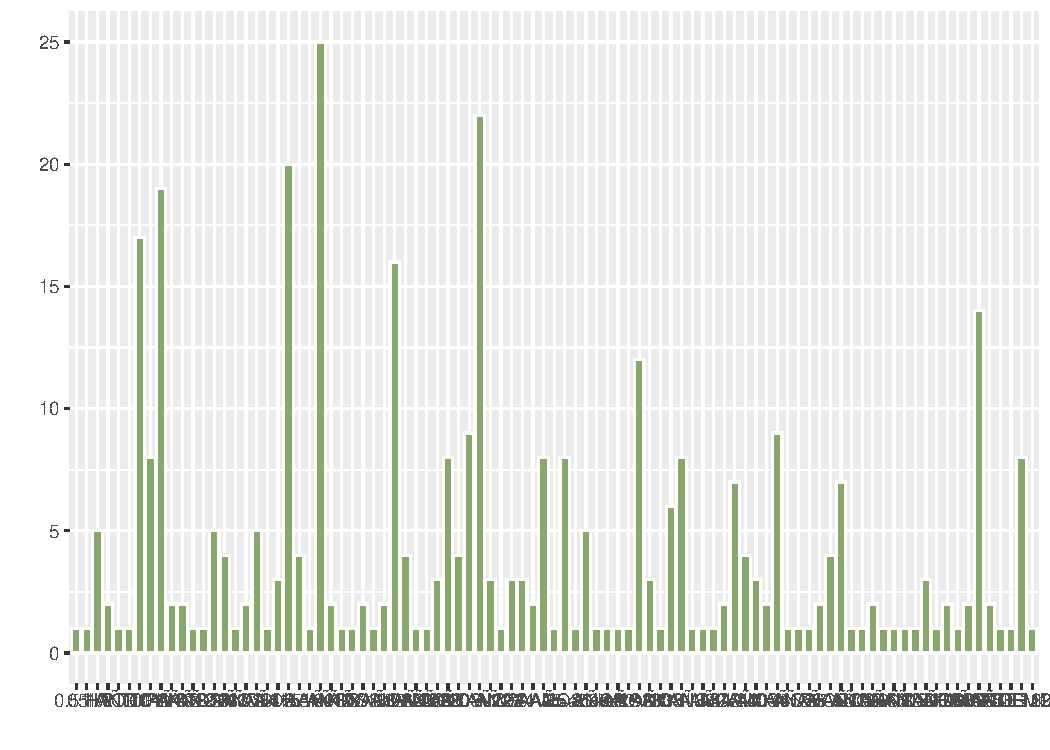
\includegraphics[width=\maxwidth]{figure/fig_diecinueve-1} 
\end{knitrout}
}
\end{graficas}

%\begin{fotos}
%{reconocimiento en campo}{17}
%\end{fotos}
\end{comment}

\begin{tablas}
{Fuente del agua para riego}{

\begin{tabular}{lcl}
\toprule
\cellcolor[HTML]{87A96B}{\textcolor{black}{\textbf{Fuente\_riego}}} & \cellcolor[HTML]{87A96B}{\textcolor{black}{\textbf{Conteo}}} & \cellcolor[HTML]{87A96B}{\textcolor{black}{\textbf{Porcentaje}}}\\
\midrule
LAGO O LAGUNA & 2 & 0.45\\
MANANTIAL & 217 & 48.55\\
OTRO & 18 & 4.03\\
POZOS & 1 & 0.22\\
RIO & 209 & 46.76\\
\bottomrule
\end{tabular}


}
\end{tablas}
\begin{graficas}
{Fuente del agua para riego}{
\begin{knitrout}
\definecolor{shadecolor}{rgb}{0.969, 0.969, 0.969}\color{fgcolor}
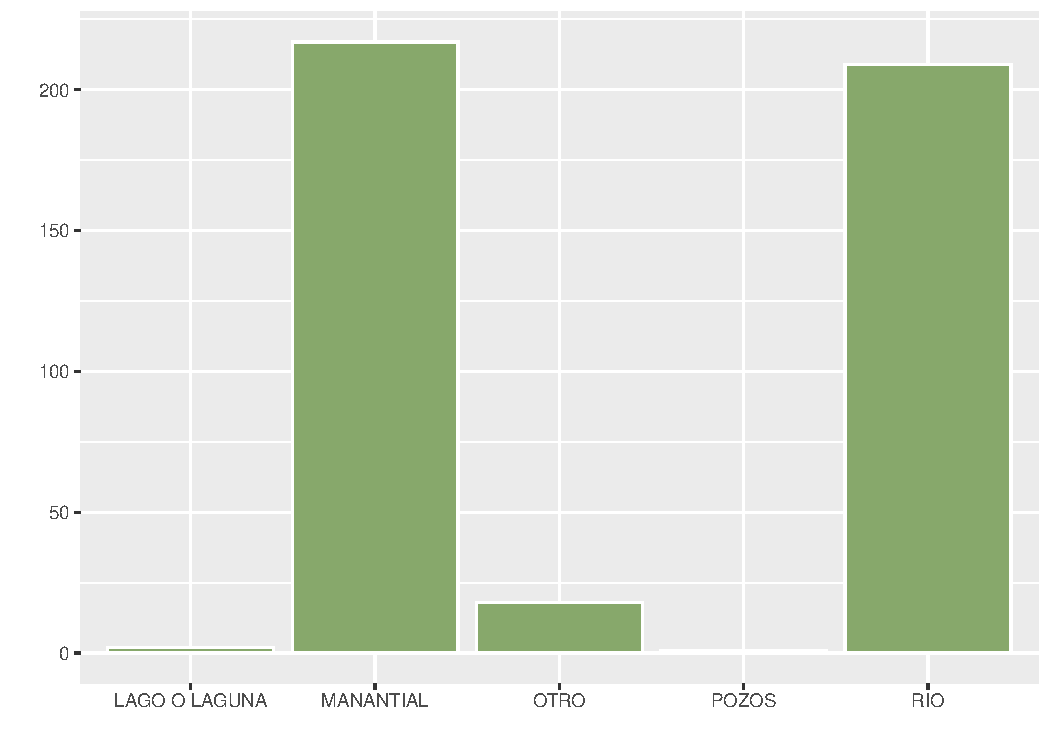
\includegraphics[width=\maxwidth]{figure/fig_veinte-1} 
\end{knitrout}
}
\end{graficas}
La tabla presentada indica que el 48.55\% de los agricultores utiliza manantiales como su principal fuente de agua para riego, lo que señala una considerable dependencia de fuentes naturales, las cuales pueden ser susceptibles a variaciones climáticas y estacionales, lo que podría afectar la estabilidad de la producción agrícola, un 46.76\% de los usuarios encuestados hace uso de ríos, lo que sugiere que una parte significativa de la actividad agrícola depende de cuerpos de agua superficiales, si bien esto puede ofrecer ventajas en cuanto a acceso, también provoca riesgos relacionados con la contaminación y fluctuaciones en el caudal, por otro lado, el empleo de pozos (0.45\%) y lagos o lagunas (0.22\%) es muy bajo, lo que indica que los agricultores no están aprovechando de manera óptima estas fuentes alternativas, lo cual podría restringir su capacidad para diversificar las fuentes de agua y asegurar el riego en períodos de escasez. En conclusión, la fuerte dependencia de manantiales y ríos para el riego subraya la necesidad urgente de implementar prácticas de gestión sostenible del agua, a fin de asegurar la productividad agrícola a largo plazo, particularmente ante la amenaza del cambio climático.
\begin{fotos}
{reconocimiento en campo}{18}
\end{fotos}

\begin{comment}
\begin{tablas}
{Fuente de agua para riego}{

\begin{tabular}{lcl}
\toprule
\cellcolor[HTML]{87A96B}{\textcolor{black}{\textbf{Fuente\_riego}}} & \cellcolor[HTML]{87A96B}{\textcolor{black}{\textbf{Conteo}}} & \cellcolor[HTML]{87A96B}{\textcolor{black}{\textbf{Porcentaje}}}\\
\midrule
LAGO O LAGUNA & 2 & 0.45\\
MANANTIAL & 217 & 48.55\\
OTRO & 18 & 4.03\\
POZOS & 1 & 0.22\\
RIO & 209 & 46.76\\
\bottomrule
\end{tabular}


}
\end{tablas}
\begin{graficas}
{Fuente de agua para riego}{
\begin{knitrout}
\definecolor{shadecolor}{rgb}{0.969, 0.969, 0.969}\color{fgcolor}
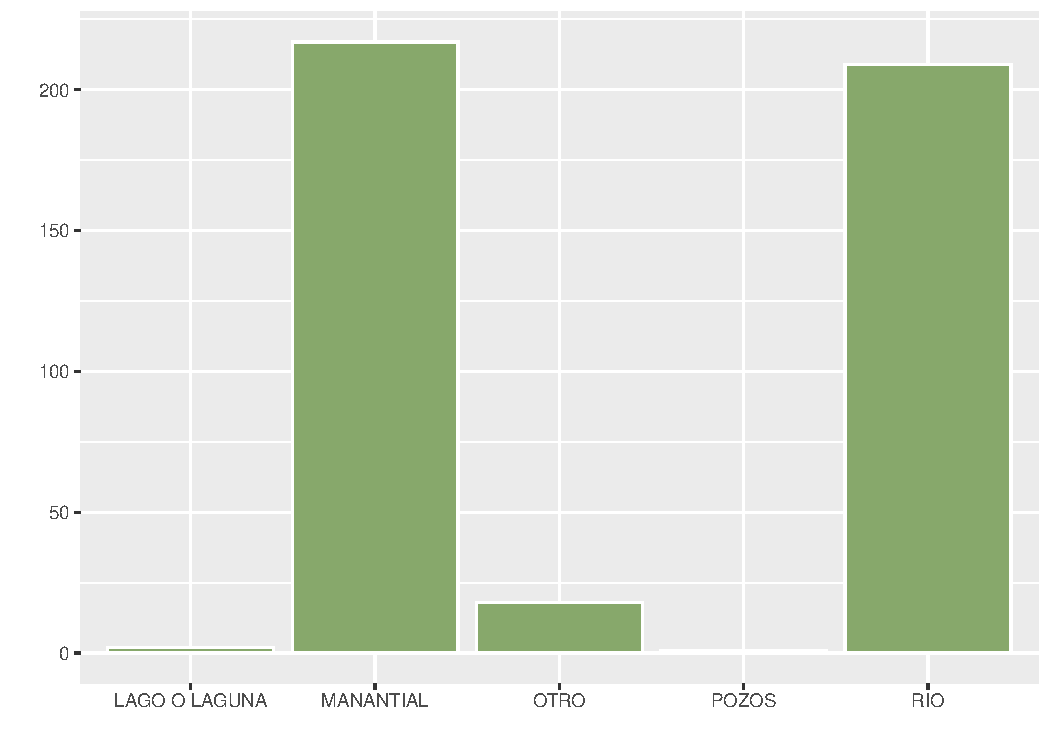
\includegraphics[width=\maxwidth]{figure/fig_veintiuno-1} 
\end{knitrout}
}
\end{graficas}
%\begin{fotos}
%{reconocimiento en campo}{19}
%\end{fotos}
\end{comment}

\begin{tablas}
{Frecuencia de riego de la parcela}{

\begin{tabular}{lcl}
\toprule
\cellcolor[HTML]{87A96B}{\textcolor{black}{\textbf{Frecuencia\_riego}}} & \cellcolor[HTML]{87A96B}{\textcolor{black}{\textbf{Conteo}}} & \cellcolor[HTML]{87A96B}{\textcolor{black}{\textbf{Porcentaje}}}\\
\midrule
OTRO & 31 & 7.01\\
POR DIAS & 83 & 18.78\\
POR HORAS & 20 & 4.52\\
POR TURNOS & 305 & 69.00\\
POR VOLUMEN & 3 & 0.68\\
\bottomrule
\end{tabular}


}
\end{tablas}
\begin{graficas}
{Frecuencia de riego de la parcela}{
\begin{knitrout}
\definecolor{shadecolor}{rgb}{0.969, 0.969, 0.969}\color{fgcolor}
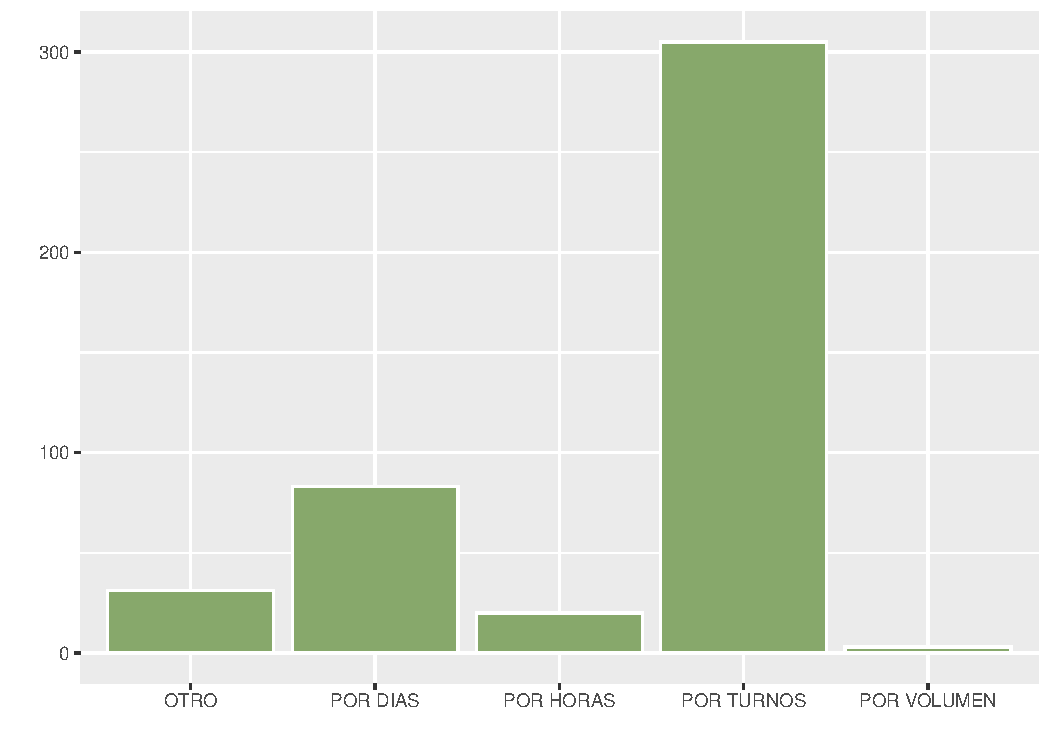
\includegraphics[width=\maxwidth]{figure/fig_veintidos-1} 
\end{knitrout}
}
\end{graficas}
La tabla muestra la frecuencia de riego de la parcela, el riego por turnos se utiliza en un 69\% es el método más utilizado por los agricultores, lo que sugiere una gestión más controlada y eficiente del recurso hídrico, favoreciendo así la productividad agrícola al permitir un uso más preciso del agua, en segundo lugar el 18.78\% de los agricultores emplea riego por días, lo que puede reflejar un enfoque más tradicional, pero potencialmente menos eficiente, ya que no se ajusta de manera flexible a las necesidades específicas de los cultivos o las condiciones climáticas y los métodos como el riego por horas (7.01\%) y el riego por turnos (4.52\%) son menos comunes ,aunque pueden ser útiles en ciertos contextos, presentan desafíos para una gestión eficiente del agua, por último  el 0.68\% de los agricultores utiliza el riego por volumen, una categoría que podría señalar la existencia de enfoques alternativos menos estandarizados. En general, aunque el riego por turnos parece ser el más beneficioso para optimizar el uso del agua, es crucial que los agricultores exploren y adopten métodos más eficientes y sostenibles para enfrentar los retos relacionados con la escasez de agua y garantizar una producción agrícola.
\begin{fotos}
{reconocimiento en campo}{20}
\end{fotos}

\begin{tablas}
{Infraestructura de riego}{

\begin{tabular}{lcl}
\toprule
\cellcolor[HTML]{87A96B}{\textcolor{black}{\textbf{Tipo\_infraestructura}}} & \cellcolor[HTML]{87A96B}{\textcolor{black}{\textbf{Conteo}}} & \cellcolor[HTML]{87A96B}{\textcolor{black}{\textbf{Porcentaje}}}\\
\midrule
REBESTIDO & 259 & 72.35\\
TAJO ABIERTO & 99 & 27.65\\
\bottomrule
\end{tabular}


}
\end{tablas}
\begin{graficas}
{Infraestructura de riego}{
\begin{knitrout}
\definecolor{shadecolor}{rgb}{0.969, 0.969, 0.969}\color{fgcolor}
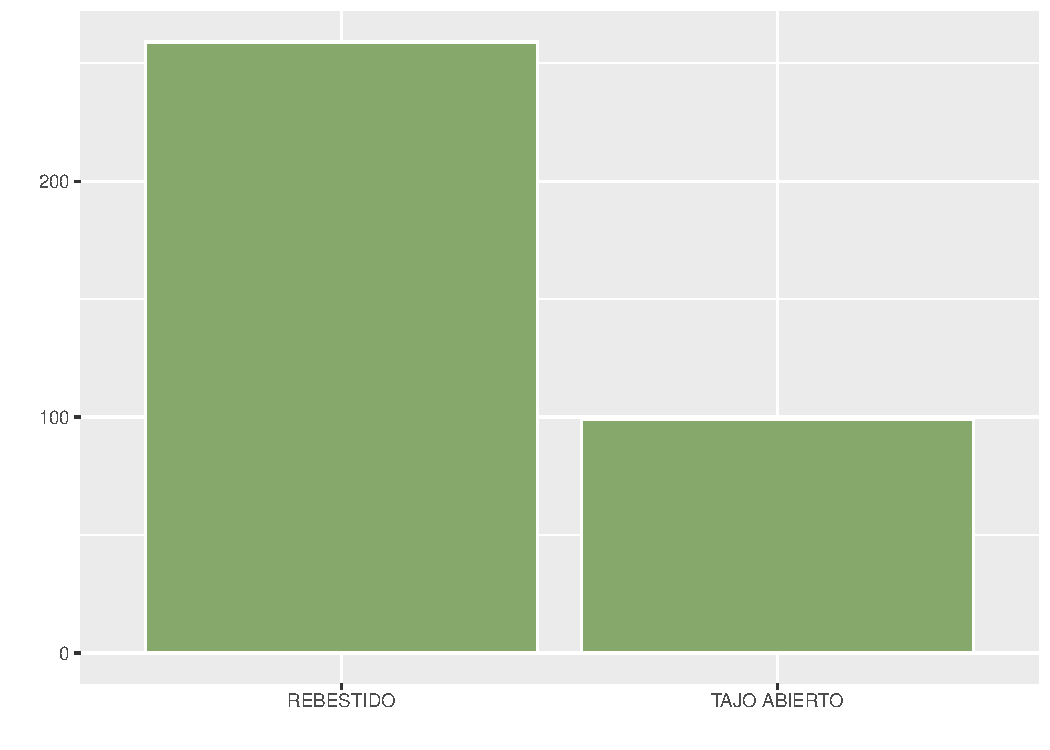
\includegraphics[width=\maxwidth]{figure/fig_veintitres-1} 
\end{knitrout}
}
\end{graficas}
La tabla indica que el 72.35\% de la infraestructura de riego empleada es de revestido, lo que indica que la mayoría de los agricultores utilizan sistemas más avanzados, probablemente más eficientes, lo que puede favorecer una mejor gestión del agua y, en consecuencia, aumentar la productividad agrícola, en cambio el 27.65\% de los encuestados emplea riego a tajo abierto, un método menos eficiente que tiende a generar mayores pérdidas de agua por evaporación, lo que podría restringir la capacidad de los agricultores para optimizar sus cosechas. En conclusion, la alta proporción de infraestructura de revestido es un aspecto positivo para la productividad agrícola, pero es crucial seguir invirtiendo en el perfeccionamiento de las prácticas de riego para asegurar una gestión más efectiva de los recursos hídricos y fomentar una agricultura más sostenible


\begin{fotos}
{reconocimiento en campo}{21}
\end{fotos}


\begin{tablas}
{Tipo de riego que utiliza}{

\begin{tabular}{lcl}
\toprule
\cellcolor[HTML]{87A96B}{\textcolor{black}{\textbf{Tipo\_riego}}} & \cellcolor[HTML]{87A96B}{\textcolor{black}{\textbf{Conteo}}} & \cellcolor[HTML]{87A96B}{\textcolor{black}{\textbf{Porcentaje}}}\\
\midrule
OTRO & 9 & 2.04\\
POR GRAVEDAD & 43 & 9.73\\
POZO O AGUA SUBTERRANEA & 1 & 0.23\\
TECNIFICADO & 389 & 88.01\\
\bottomrule
\end{tabular}


}
\end{tablas}
\begin{graficas}
{Tipo de riego que utiliza}{
\begin{knitrout}
\definecolor{shadecolor}{rgb}{0.969, 0.969, 0.969}\color{fgcolor}
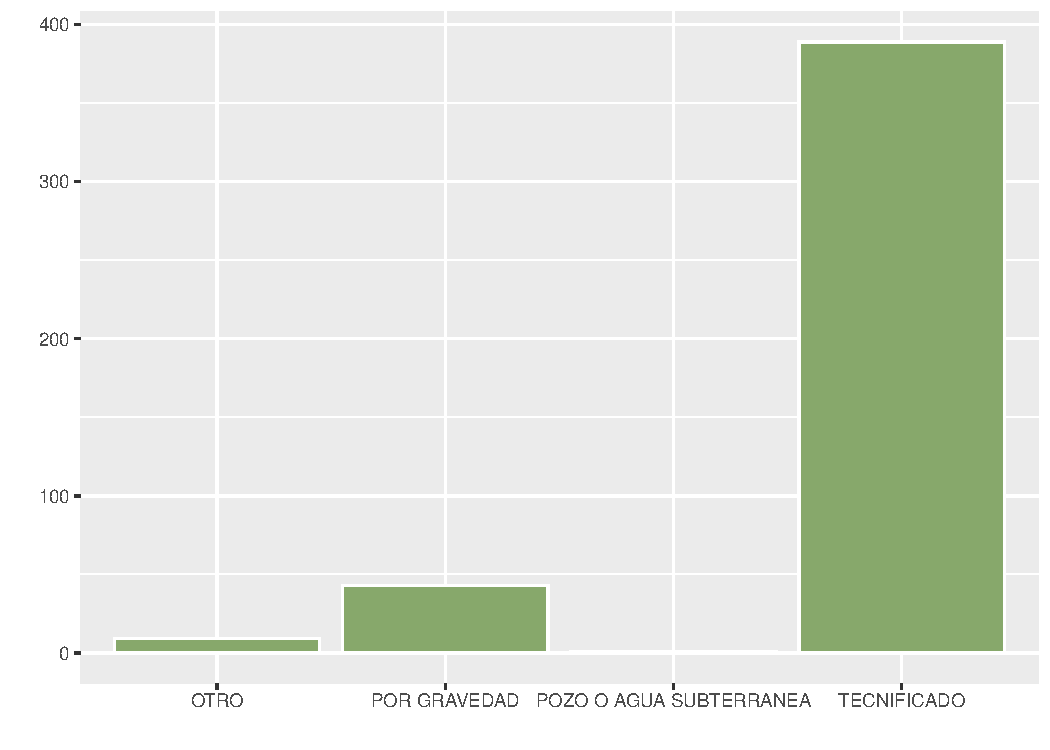
\includegraphics[width=\maxwidth]{figure/fig_veinticuatro-1} 
\end{knitrout}
}
\end{graficas}
La tabla indica que el 88.01\% de los agricultores utiliza riego tecnificado, lo que refleja que este método sigue siendo el más común en la región, sin embargo también sugiere que la adopción de tecnologías más avanzadas es limitada, lo que podría ser un obstáculo para mejorar la eficiencia en el uso del agua y aumentar los rendimientos agrícolas, en cambio solo el 0.23\% de los agricultores recurre al uso de agua subterránea mediante pozos, mientras que el 9.73\% prefiere el riego por gravedad, un sistema tradicional que, aunque puede funcionar bien en ciertos terrenos, tiene limitaciones en cuanto a la eficiencia hídrica, este método no permite un control exacto sobre la cantidad de agua utilizada, lo que puede resultar en desperdicio y un uso ineficiente del recurso en la categoría otro el 0.23\% de usuarios encuestados sugiere que existen prácticas aún menos frecuentes, lo que refuerza la idea de que la mayoría de los agricultores sigue utilizando métodos tradicionales, lo que podría restringir su capacidad para adaptarse a cambios en el clima o mejorar su productividad. El análisis muestra que, a pesar de que el riego tecnificado es la opción predominante, su adopción limitada indica una posible brecha tecnológica que impide a muchos agricultores aprovechar al máximo los beneficios de métodos más precisos y eficientes en el uso del agua.
\begin{fotos}
{reconocimiento en campo}{22}
\end{fotos}


\begin{tablas}
{Pago por uso de agua para riego}{

\begin{tabular}{lcl}
\toprule
\cellcolor[HTML]{87A96B}{\textcolor{black}{\textbf{Pago\_agua}}} & \cellcolor[HTML]{87A96B}{\textcolor{black}{\textbf{Conteo}}} & \cellcolor[HTML]{87A96B}{\textcolor{black}{\textbf{Porcentaje}}}\\
\midrule
NO & 27 & 6.15\\
SI & 412 & 93.85\\
\bottomrule
\end{tabular}


}
\end{tablas}
\begin{graficas}
{Pago por uso de agua para riego}{
\begin{knitrout}
\definecolor{shadecolor}{rgb}{0.969, 0.969, 0.969}\color{fgcolor}
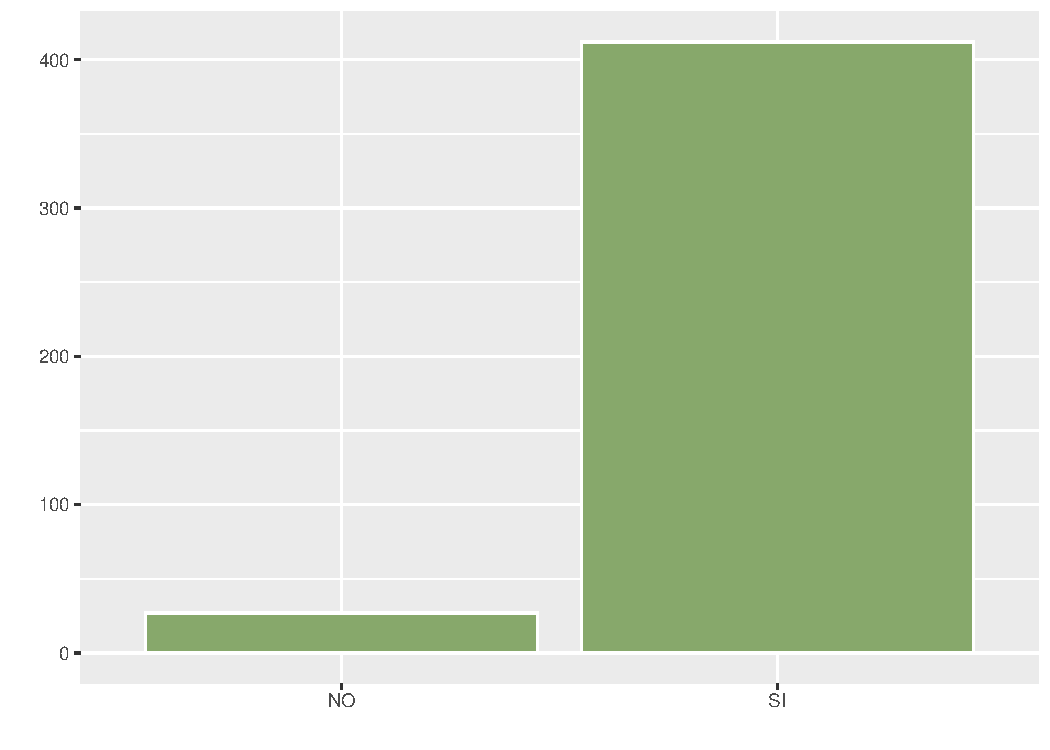
\includegraphics[width=\maxwidth]{figure/fig_veinticinco-1} 
\end{knitrout}
}
\end{graficas}
La Tabla muestra que un 93.85\% de los agricultores paga por el uso del agua para riego, lo que indica una alta dependencia de este recurso y una conciencia sobre su valor, esto sugiere que el costo del agua podría fomentar la adopción de prácticas más sostenibles y eficientes en su utilización, solo el 6.15\% no realiza ningún tipo de pago, lo que podría implicar que estos agricultores tienen acceso a fuentes de agua gratuitas o no reguladas, lo que podría llevar a una gestión menos responsable del recurso. En conclusión, la elevada proporción de agricultores que paga por el uso de agua representa una oportunidad para fomentar la gestión responsable del agua, un factor esencial para maximizar la productividad agrícola en un contexto de creciente escasez de recursos hídricos.
\begin{fotos}
{reconocimiento en campo}{23}
\end{fotos}


\begin{tablas}
{Frecuencia por uso de agua para riego}{

\begin{tabular}{lcl}
\toprule
\cellcolor[HTML]{87A96B}{\textcolor{black}{\textbf{Frecuencia\_pago}}} & \cellcolor[HTML]{87A96B}{\textcolor{black}{\textbf{Conteo}}} & \cellcolor[HTML]{87A96B}{\textcolor{black}{\textbf{Porcentaje}}}\\
\midrule
ANUAL & 348 & 85.93\\
DIARIO & 24 & 5.93\\
MENSUAL & 18 & 4.44\\
QUINCENAL & 6 & 1.48\\
SEMESTRAL & 9 & 2.22\\
\bottomrule
\end{tabular}


}
\end{tablas}
\begin{graficas}
{Frecuencia por uso de agua para riego}{
\begin{knitrout}
\definecolor{shadecolor}{rgb}{0.969, 0.969, 0.969}\color{fgcolor}
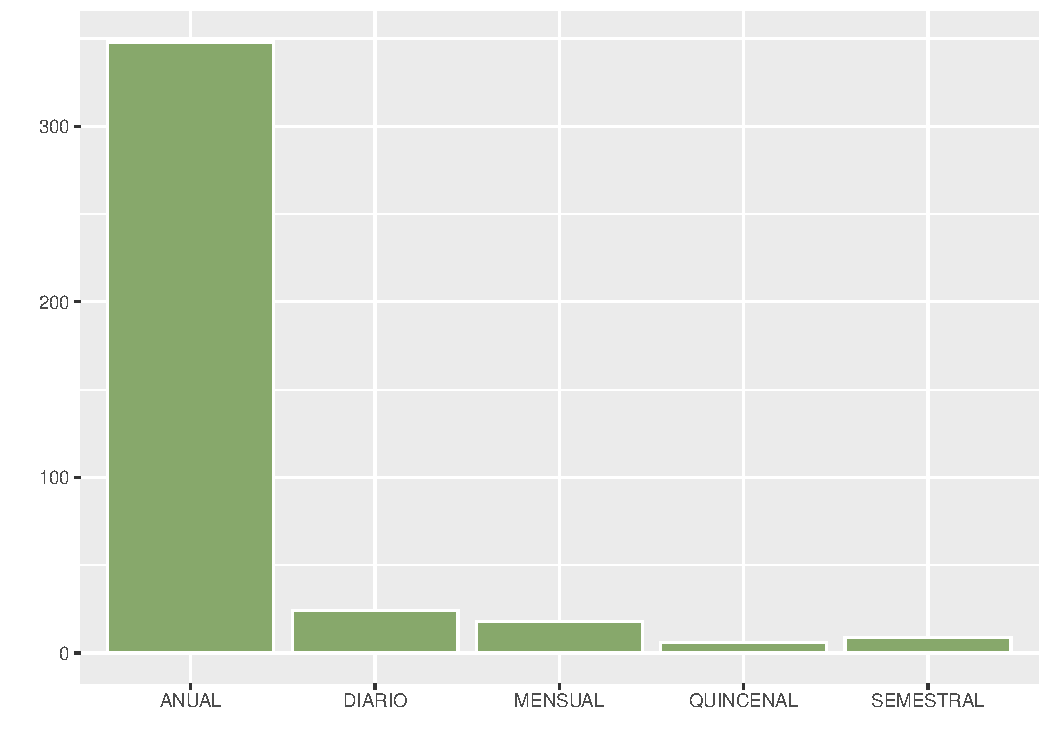
\includegraphics[width=\maxwidth]{figure/fig_veintiseis-1} 
\end{knitrout}
}
\end{graficas}
\begin{fotos}
{reconocimiento en campo}{24}
\end{fotos}


\begin{tablas}
{Derecho de uso de agua}{

\begin{tabular}{lcl}
\toprule
\cellcolor[HTML]{87A96B}{\textcolor{black}{\textbf{Derecho}}} & \cellcolor[HTML]{87A96B}{\textcolor{black}{\textbf{Conteo}}} & \cellcolor[HTML]{87A96B}{\textcolor{black}{\textbf{Porcentaje}}}\\
\midrule
NO & 6 & 1.36\\
SI & 434 & 98.64\\
\bottomrule
\end{tabular}


}
\end{tablas}
\begin{graficas}
{Derecho de uso de agua}{
\begin{knitrout}
\definecolor{shadecolor}{rgb}{0.969, 0.969, 0.969}\color{fgcolor}
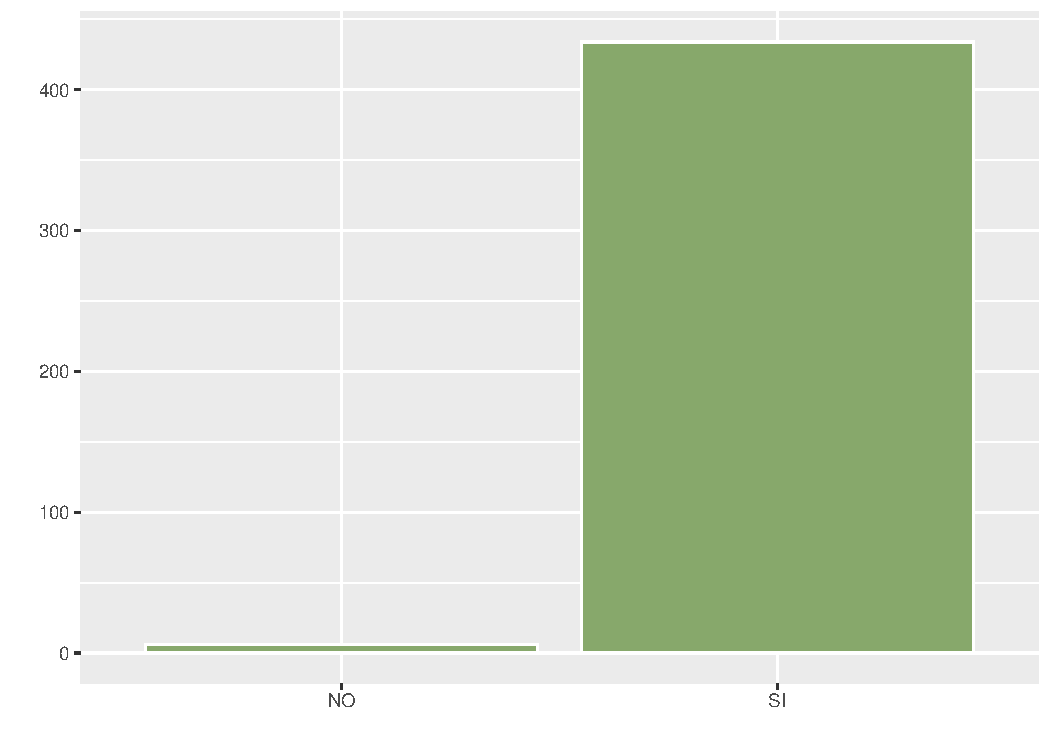
\includegraphics[width=\maxwidth]{figure/fig_veintisiete-1} 
\end{knitrout}
}
\end{graficas}
\begin{fotos}
{aplicacion de encuesta}{25}
\end{fotos}


\begin{tablas}
{Produccion predominante}{

\begin{tabular}{lcl}
\toprule
\cellcolor[HTML]{87A96B}{\textcolor{black}{\textbf{Cultivo}}} & \cellcolor[HTML]{87A96B}{\textcolor{black}{\textbf{Conteo}}} & \cellcolor[HTML]{87A96B}{\textcolor{black}{\textbf{Porcentaje}}}\\
\midrule
HORTALIZAS & 9 & 2.03\\
MAIZ CHOCLO & 40 & 9.03\\
MAIZ CHOCLO, HORTALIZAS & 7 & 1.58\\
MAIZ CHOCLO, HORTALIZAS, OTRO & 1 & 0.23\\
MAIZ CHOCLO, OTRO & 2 & 0.45\\
\addlinespace
OTRO & 2 & 0.45\\
PAPA & 12 & 2.71\\
PAPA, HORTALIZAS & 1 & 0.23\\
PAPA, MAIZ CHOCLO & 47 & 10.61\\
PAPA, MAIZ CHOCLO, HORTALIZAS & 10 & 2.26\\
\addlinespace
PAPA, MAIZ CHOCLO, HORTALIZAS, OTRO & 1 & 0.23\\
PAPA, MAIZ CHOCLO, OTRO & 1 & 0.23\\
PAPA, OTRO & 1 & 0.23\\
PASTOS & 60 & 13.54\\
PASTOS, HORTALIZAS & 1 & 0.23\\
\addlinespace
PASTOS, MAIZ CHOCLO & 5 & 1.13\\
PASTOS, MAIZ CHOCLO, HORTALIZAS & 1 & 0.23\\
PASTOS, PAPA & 7 & 1.58\\
PASTOS, PAPA, HORTALIZAS & 27 & 6.09\\
PASTOS, PAPA, HORTALIZAS, OTRO & 4 & 0.90\\
\addlinespace
PASTOS, PAPA, MAIZ CHOCLO & 50 & 11.29\\
PASTOS, PAPA, MAIZ CHOCLO, HORTALIZAS & 141 & 31.83\\
PASTOS, PAPA, MAIZ CHOCLO, HORTALIZAS, OTRO & 5 & 1.13\\
PASTOS, PAPA, MAIZ CHOCLO, OTRO & 4 & 0.90\\
PASTOS, PAPA, OTRO & 4 & 0.90\\
\bottomrule
\end{tabular}


}
\end{tablas}

\begin{graficas}
{Produccion predominante}{
\begin{knitrout}
\definecolor{shadecolor}{rgb}{0.969, 0.969, 0.969}\color{fgcolor}
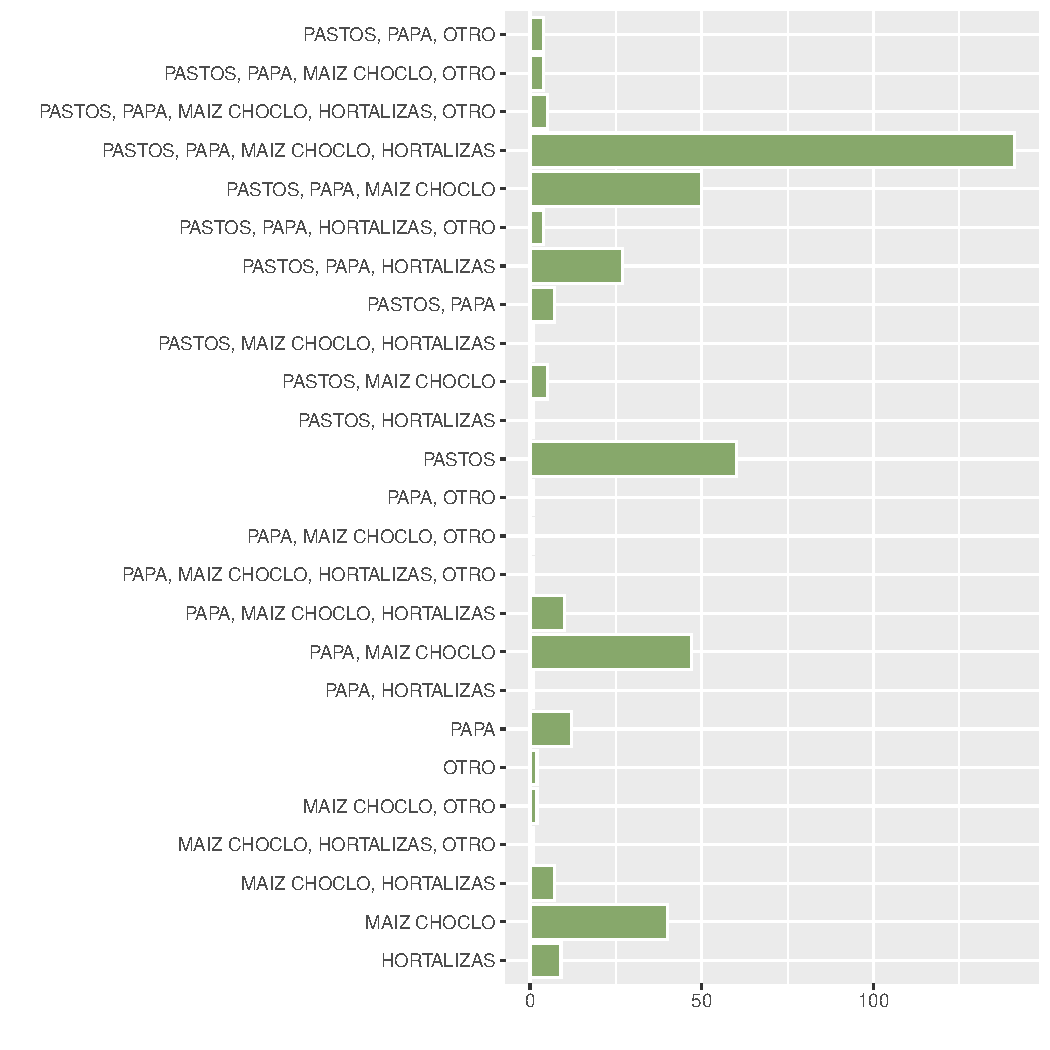
\includegraphics[width=\maxwidth]{figure/fig_veintiocho-1} 
\end{knitrout}
}
\end{graficas}

\begin{fotos}
{aplicacion de encuesta}{26}
\end{fotos}


\begin{tablas}
{Tiempo que se dedica al cultivo}{

\begin{tabular}{lcl}
\toprule
\cellcolor[HTML]{87A96B}{\textcolor{black}{\textbf{Tiempo}}} & \cellcolor[HTML]{87A96B}{\textcolor{black}{\textbf{Conteo}}} & \cellcolor[HTML]{87A96B}{\textcolor{black}{\textbf{Porcentaje}}}\\
\midrule
HACE 02 AÑOS & 3 & 0.71\\
HACE 1 AÑO & 3 & 0.71\\
MAS DE 3 AÑOS & 56 & 13.30\\
MAS DE 5 AÑOS & 359 & 85.27\\
\bottomrule
\end{tabular}


}
\end{tablas}

\begin{graficas}
{Tiempo que se dedica al cultivo}{
\begin{knitrout}
\definecolor{shadecolor}{rgb}{0.969, 0.969, 0.969}\color{fgcolor}
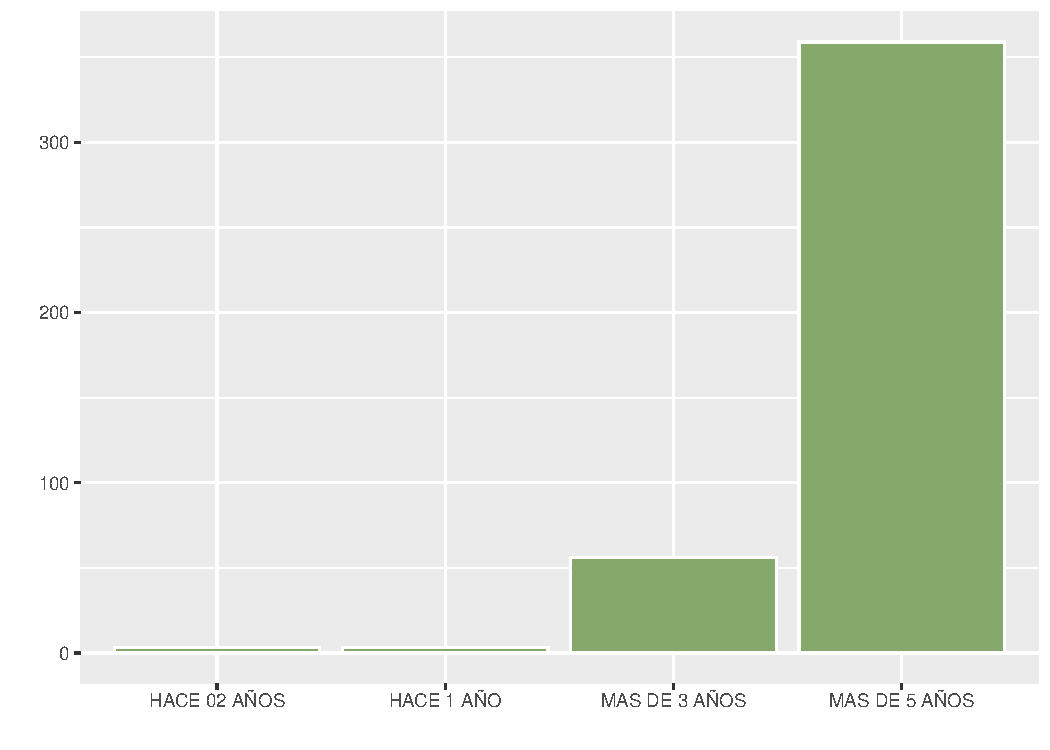
\includegraphics[width=\maxwidth]{figure/fig_veintinueve-1} 
\end{knitrout}
}
\end{graficas}

\begin{fotos}
{socializacion del proyecto}{27}
\end{fotos}


\begin{tablas}
{Finalidad de cosecha}{

\begin{tabular}{lcl}
\toprule
\cellcolor[HTML]{87A96B}{\textcolor{black}{\textbf{Finalidad}}} & \cellcolor[HTML]{87A96B}{\textcolor{black}{\textbf{Conteo}}} & \cellcolor[HTML]{87A96B}{\textcolor{black}{\textbf{Porcentaje}}}\\
\midrule
CONSUMO & 144 & 35.29\\
VENTA & 2 & 0.49\\
VENTA Y CONSUMO & 262 & 64.22\\
\bottomrule
\end{tabular}


}
\end{tablas}

\begin{graficas}
{Finalidad de cosecha}{
\begin{knitrout}
\definecolor{shadecolor}{rgb}{0.969, 0.969, 0.969}\color{fgcolor}
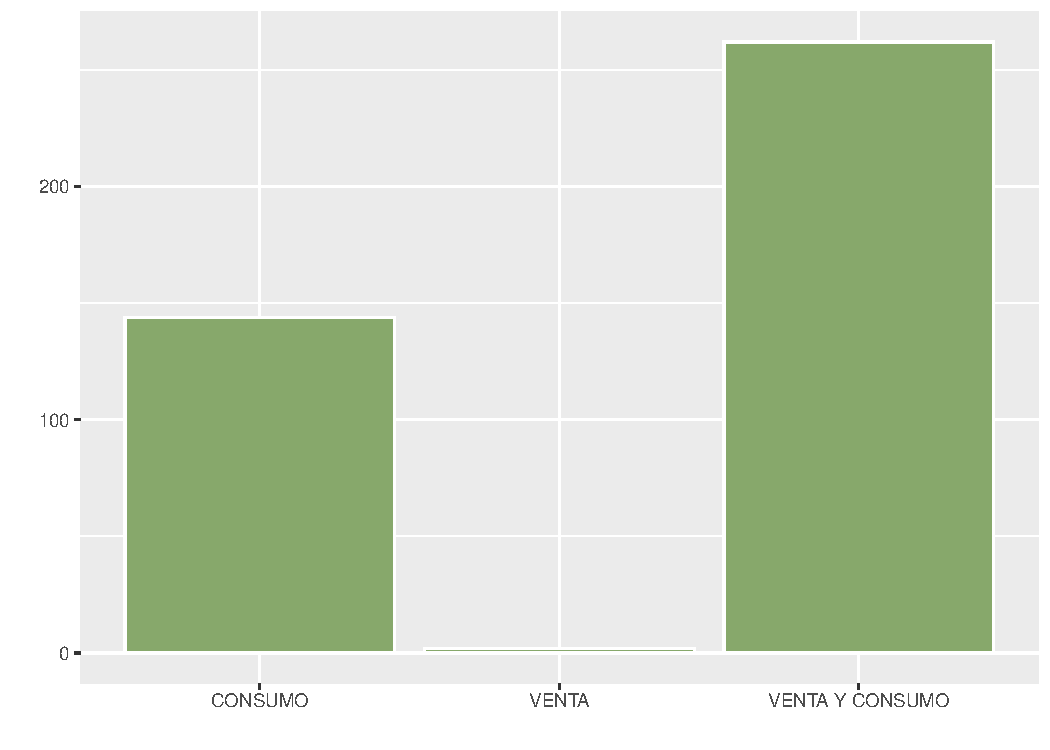
\includegraphics[width=\maxwidth]{figure/fig_treinta-1} 
\end{knitrout}
}
\end{graficas}

\begin{fotos}
{socializacion del proyecto}{28}
\end{fotos}


\begin{tablas}
{Causas que ocasionan la disminucion de la produccion de cultivo}{

\begin{tabular}{lcl}
\toprule
\cellcolor[HTML]{87A96B}{\textcolor{black}{\textbf{Causas}}} & \cellcolor[HTML]{87A96B}{\textcolor{black}{\textbf{Conteo}}} & \cellcolor[HTML]{87A96B}{\textcolor{black}{\textbf{Porcentaje}}}\\
\midrule
FACTORES ADVERSOS & 22 & 5.07\\
FALTA DE AGUA & 24 & 5.53\\
FALTA DE AGUA Y FACTORES ADVERSOS & 100 & 23.04\\
FALTA DE AGUA, FACTORES ADVERSOS Y SUELOS POBRES & 267 & 61.52\\
FALTA DE AGUA, SUELOS PROBRES Y ERIAZOS & 7 & 1.61\\
\addlinespace
SUELOS POBRES & 5 & 1.15\\
SUELOS POBRES Y FACTORES ADVERSOS & 9 & 2.07\\
\bottomrule
\end{tabular}


}
\end{tablas}

\begin{graficas}
{Causas que ocasionan la disminucion de la produccion de cultivo}{
\begin{knitrout}
\definecolor{shadecolor}{rgb}{0.969, 0.969, 0.969}\color{fgcolor}
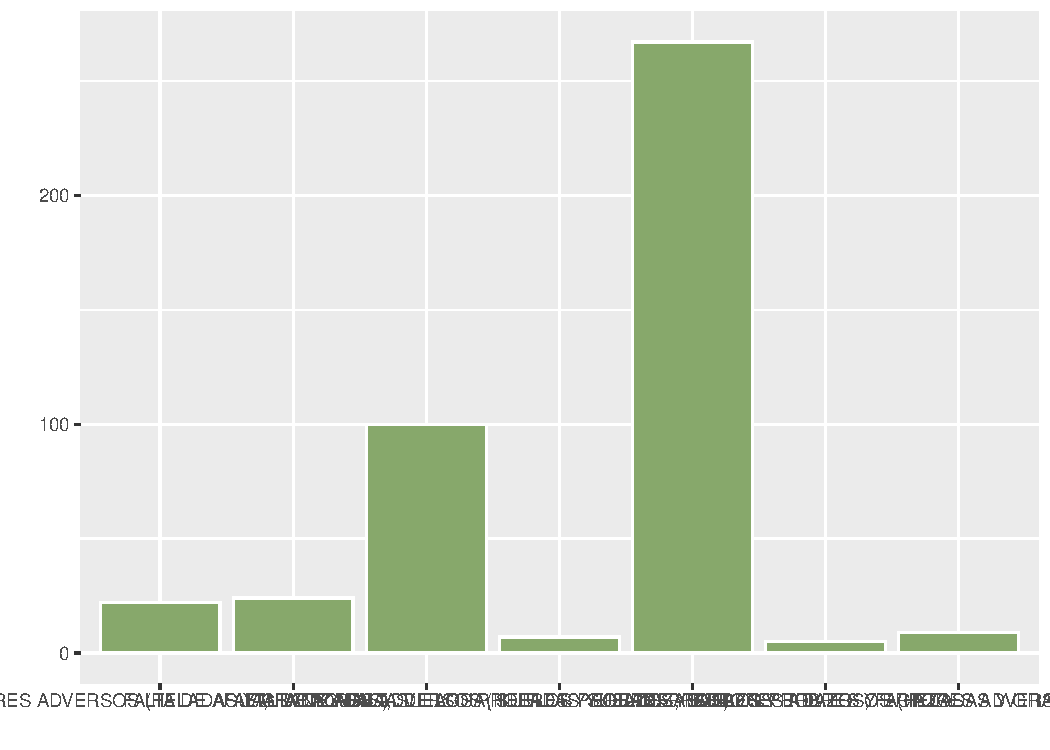
\includegraphics[width=\maxwidth]{figure/fig_treintayuno-1} 
\end{knitrout}
}
\end{graficas}

\begin{fotos}
{socializacion del proyecto}{29}
\end{fotos}

\begin{tablas}
{Registra la venta de su produccion}{

\begin{tabular}{lcl}
\toprule
\cellcolor[HTML]{87A96B}{\textcolor{black}{\textbf{Registo\_ventas}}} & \cellcolor[HTML]{87A96B}{\textcolor{black}{\textbf{Conteo}}} & \cellcolor[HTML]{87A96B}{\textcolor{black}{\textbf{Porcentaje}}}\\
\midrule
NO & 162 & 40.5\\
SI & 238 & 59.5\\
\bottomrule
\end{tabular}


}
\end{tablas}

\begin{graficas}
{Registra la venta de su produccion}{
\begin{knitrout}
\definecolor{shadecolor}{rgb}{0.969, 0.969, 0.969}\color{fgcolor}
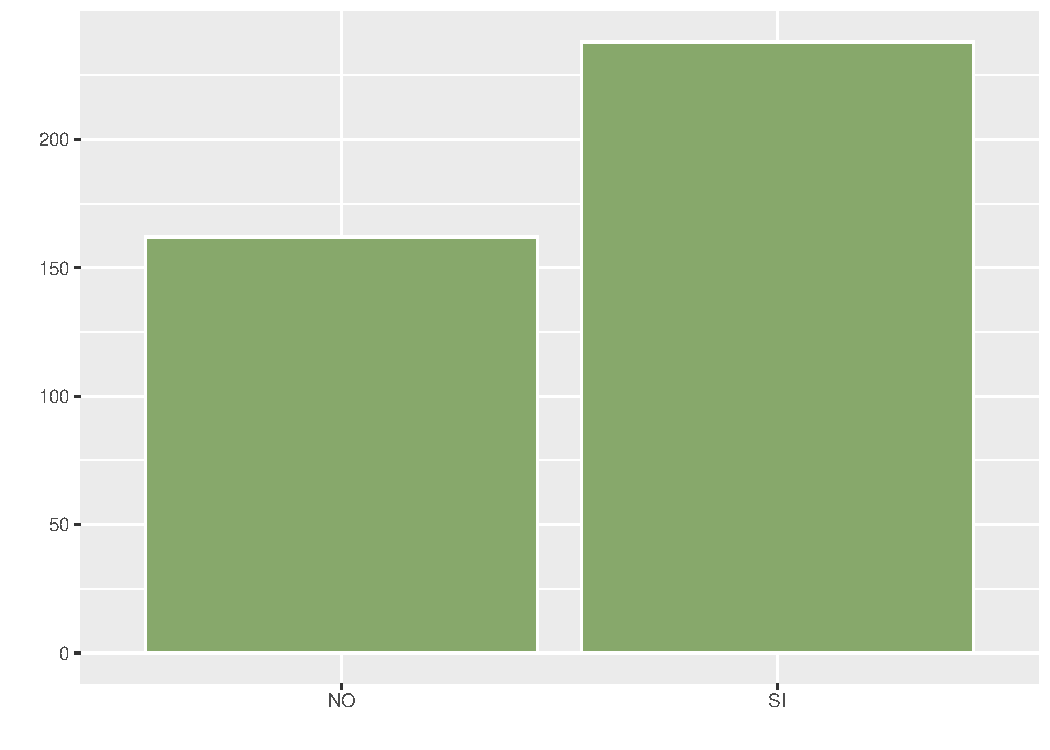
\includegraphics[width=\maxwidth]{figure/fig_treintaydos-1} 
\end{knitrout}
}
\end{graficas}

\begin{fotos}
{socializacion del proyecto}{30}
\end{fotos}

\begin{tablas}
{Personas con las que realiza la cosecha}{

\begin{tabular}{lcl}
\toprule
\cellcolor[HTML]{87A96B}{\textcolor{black}{\textbf{Personas}}} & \cellcolor[HTML]{87A96B}{\textcolor{black}{\textbf{Conteo}}} & \cellcolor[HTML]{87A96B}{\textcolor{black}{\textbf{Porcentaje}}}\\
\midrule
AMIGOS & 3 & 0.78\\
FAMILIARES & 329 & 85.01\\
JORNAL & 30 & 7.75\\
OTRO & 3 & 0.78\\
SOCIOS & 1 & 0.26\\
\addlinespace
SOLO & 21 & 5.43\\
\bottomrule
\end{tabular}


}
\end{tablas}

\begin{graficas}
{Personas con las que realiza la cosecha}{
\begin{knitrout}
\definecolor{shadecolor}{rgb}{0.969, 0.969, 0.969}\color{fgcolor}
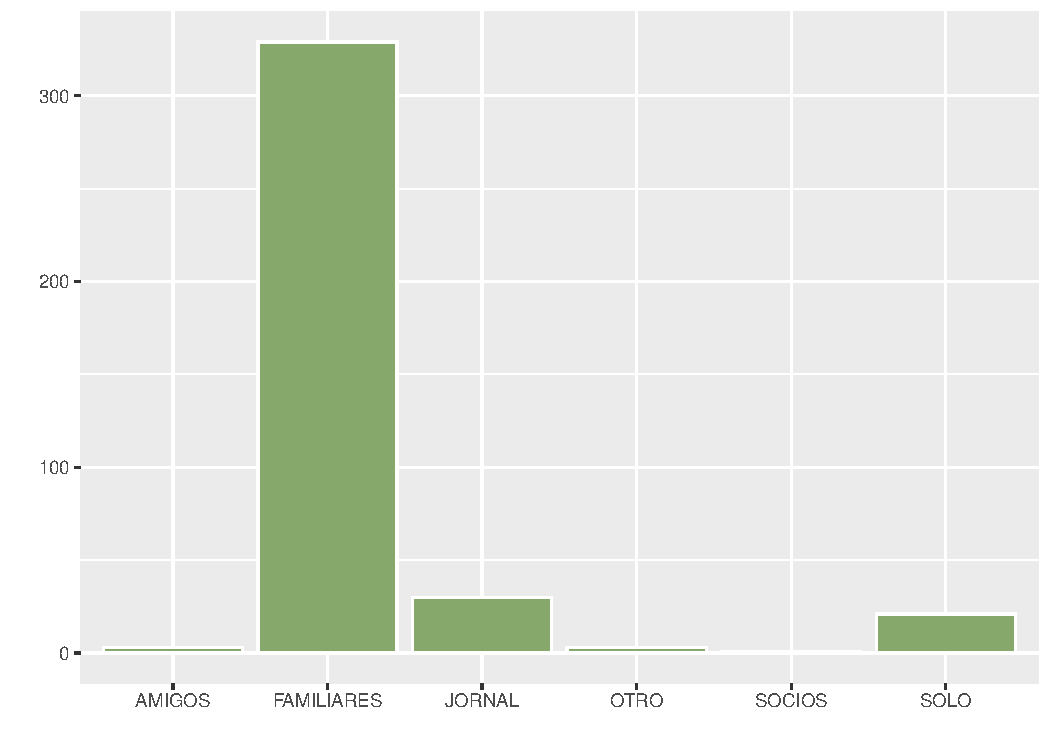
\includegraphics[width=\maxwidth]{figure/fig_treintaytres-1} 
\end{knitrout}
}
\end{graficas}

\begin{fotos}
{socializacion del proyecto}{31}
\end{fotos}


\begin{tablas}
{Practica de conservacion de suelos}{

\begin{tabular}{lcl}
\toprule
\cellcolor[HTML]{87A96B}{\textcolor{black}{\textbf{Personas}}} & \cellcolor[HTML]{87A96B}{\textcolor{black}{\textbf{Conteo}}} & \cellcolor[HTML]{87A96B}{\textcolor{black}{\textbf{Porcentaje}}}\\
\midrule
ABONOS ORGANICO Y MATERIA ORGANICA & 37 & 10.00\\
INCORPORACION EN MATERIA ORGANICA & 4 & 1.08\\
OTRO & 1 & 0.27\\
ROTACION DE CULTIVOS & 22 & 5.95\\
ROTACION DE CULTIVOS, USO DE ABONOS ORGANICOS & 129 & 34.86\\
\addlinespace
ROTACION Y MATERIA ORGANICA & 18 & 4.86\\
ROTACION, ABONO ORGANICO Y CAL & 2 & 0.54\\
ROTACION, ABONO ORGANICO, CAL Y MATERIA ORGANICA & 8 & 2.16\\
ROTACION, ABONOS ORGANICO Y MATERIA ORGANICA & 81 & 21.89\\
USO DE ABONOS ORGANICOS & 68 & 18.38\\
\bottomrule
\end{tabular}


}
\end{tablas}

\begin{graficas}
{Practica de conservacion de suelos}{
\begin{knitrout}
\definecolor{shadecolor}{rgb}{0.969, 0.969, 0.969}\color{fgcolor}
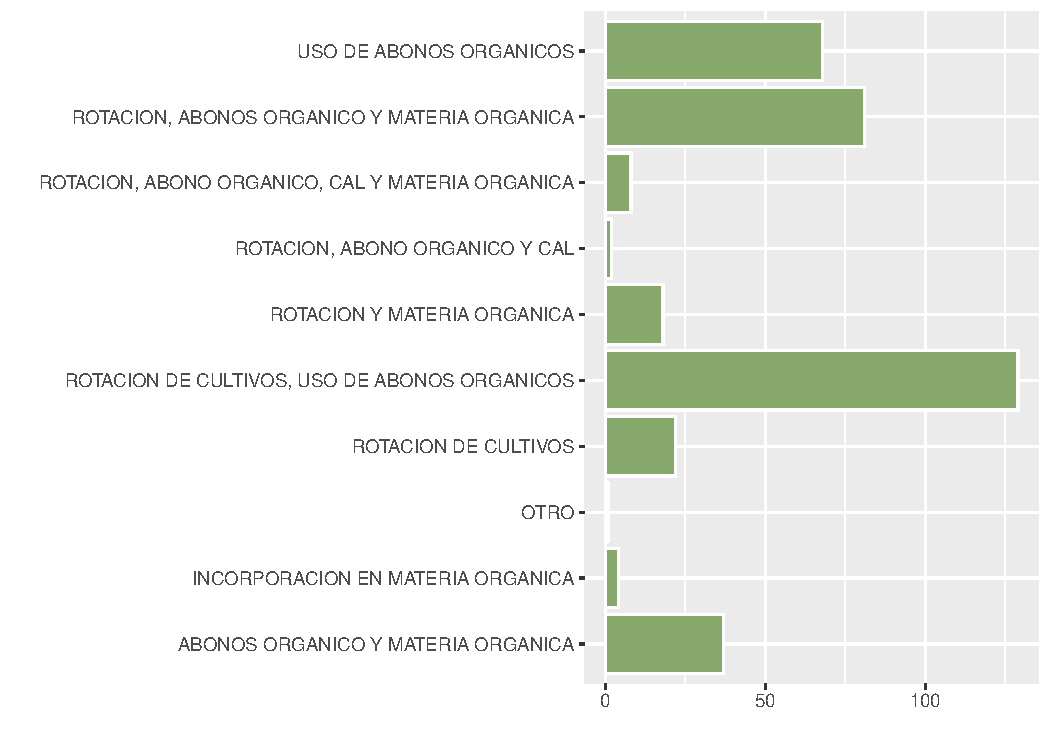
\includegraphics[width=\maxwidth]{figure/fig_treintaycuatro-1} 
\end{knitrout}
}
\end{graficas}

\begin{fotos}
{socializacion del proyecto}{32}
\end{fotos}


\begin{tablas}
{Realiza manejo de post cosecha}{

\begin{tabular}{lcl}
\toprule
\cellcolor[HTML]{87A96B}{\textcolor{black}{\textbf{Manejo}}} & \cellcolor[HTML]{87A96B}{\textcolor{black}{\textbf{Conteo}}} & \cellcolor[HTML]{87A96B}{\textcolor{black}{\textbf{Porcentaje}}}\\
\midrule
NO & 229 & 55.18\\
SI & 186 & 44.82\\
\bottomrule
\end{tabular}


}
\end{tablas}

\begin{graficas}
{Realiza manejo de post cosecha}{
\begin{knitrout}
\definecolor{shadecolor}{rgb}{0.969, 0.969, 0.969}\color{fgcolor}
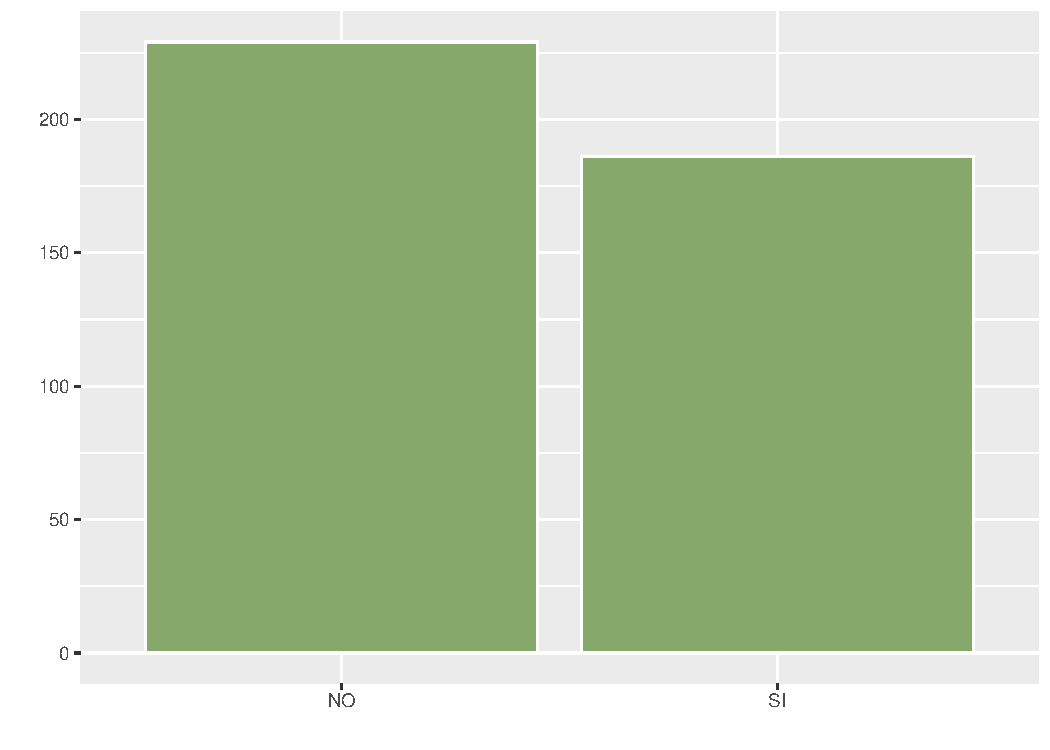
\includegraphics[width=\maxwidth]{figure/fig_treintaycinco-1} 
\end{knitrout}
}
\end{graficas}

\begin{fotos}
{socializacion del proyecto}{33}
\end{fotos}


\begin{tablas}
{Ha recibido alguna capacitacion}{

\begin{tabular}{lcl}
\toprule
\cellcolor[HTML]{87A96B}{\textcolor{black}{\textbf{Capacitacion}}} & \cellcolor[HTML]{87A96B}{\textcolor{black}{\textbf{Conteo}}} & \cellcolor[HTML]{87A96B}{\textcolor{black}{\textbf{Porcentaje}}}\\
\midrule
NO & 314 & 71.04\\
SI & 128 & 28.96\\
\bottomrule
\end{tabular}


}
\end{tablas}

\begin{graficas}
{Ha recibido alguna capacitacion}{
\begin{knitrout}
\definecolor{shadecolor}{rgb}{0.969, 0.969, 0.969}\color{fgcolor}
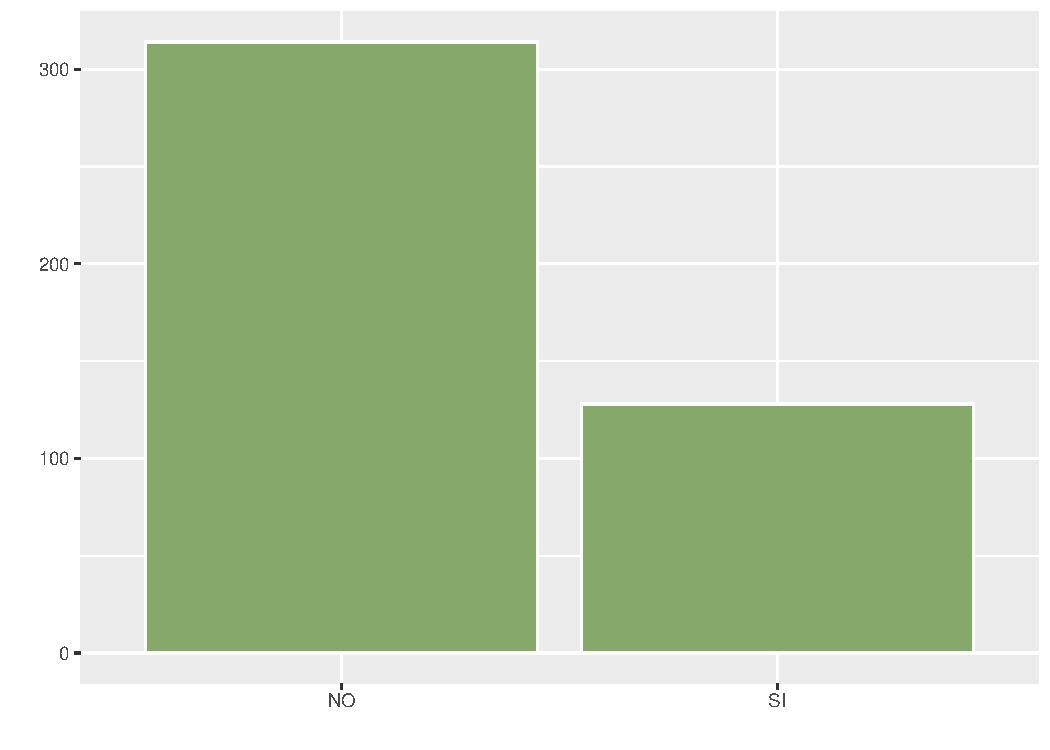
\includegraphics[width=\maxwidth]{figure/fig_treintayseis-1} 
\end{knitrout}
}
\end{graficas}

\begin{fotos}
{trabajo de campo}{34}
\end{fotos}

\begin{comment}

\begin{tablas}
{Temas de capacitacion}{

\begin{tabular}{lcl}
\toprule
\cellcolor[HTML]{87A96B}{\textcolor{black}{\textbf{Temas}}} & \cellcolor[HTML]{87A96B}{\textcolor{black}{\textbf{Conteo}}} & \cellcolor[HTML]{87A96B}{\textcolor{black}{\textbf{Porcentaje}}}\\
\midrule
CONTROL FITOSANITARIO & 2 & 1.48\\
CONTROL FITOSANITARIO, COSECHA & 1 & 0.74\\
FERTILIZACION Y ABONAMIENTO & 4 & 2.96\\
FERTILIZACION Y ABONAMIENTO, CONTROL FITOSANITARIO & 1 & 0.74\\
FERTILIZACION Y ABONAMIENTO, MEJORAMIENTO GENETICO & 1 & 0.74\\
\addlinespace
MEJORAMIENTO GENETICO & 2 & 1.48\\
OTRO & 13 & 9.63\\
PREPARACION DE TERRENO & 6 & 4.44\\
PREPARACION DE TERRENO, COSECHA & 1 & 0.74\\
PREPARACION DE TERRENO, MEJORAMIENTO GENETICO & 1 & 0.74\\
\addlinespace
PREPARACION DE TERRENO, SIEMBRA & 12 & 8.89\\
PREPARACION DE TERRENO, SIEMBRA, COSECHA & 17 & 12.59\\
PREPARACION DE TERRENO, SIEMBRA, COSECHA, MEJORAMIENTO GENETICO & 1 & 0.74\\
PREPARACION DE TERRENO, SIEMBRA, FERTILIZACION Y ABONAMIENTO & 3 & 2.22\\
PREPARACION DE TERRENO, SIEMBRA, FERTILIZACION Y ABONAMIENTO, CONTROL FITOSANITARIO & 5 & 3.70\\
\addlinespace
PREPARACION DE TERRENO, SIEMBRA, FERTILIZACION Y ABONAMIENTO, CONTROL FITOSANITARIO, COSECHA & 11 & 8.15\\
PREPARACION DE TERRENO, SIEMBRA, FERTILIZACION Y ABONAMIENTO, CONTROL FITOSANITARIO, MEJORAMIENTO GENETICO & 1 & 0.74\\
PREPARACION DE TERRENO, SIEMBRA, FERTILIZACION Y ABONAMIENTO, COSECHA & 11 & 8.15\\
PREPARACION DE TERRENO, SIEMBRA, FERTILIZACION Y ABONAMIENTO, COSECHA, MEJORAMIENTO GENETICO & 4 & 2.96\\
PREPARACION DE TERRENO, SIEMBRA, FERTILIZACION Y ABONAMIENTO, MEJORAMIENTO GENETICO & 3 & 2.22\\
\addlinespace
PREPARACION DE TERRENO, SIEMBRA, OTRO & 1 & 0.74\\
SIEMBRA & 7 & 5.19\\
SIEMBRA, CONTROL FITOSANITARIO & 1 & 0.74\\
SIEMBRA, COSECHA & 2 & 1.48\\
SIEMBRA, FERTILIZACION Y ABONAMIENTO & 1 & 0.74\\
\addlinespace
SIEMBRA, FERTILIZACION Y ABONAMIENTO, CONTROL FITOSANITARIO, COSECHA & 2 & 1.48\\
TERRENO Y FERTILIZACION & 2 & 1.48\\
TERRENO, FERTILIZACION, COSECHA & 4 & 2.96\\
TERRENO, FERTILIZACION, COSECHA, GENETICA & 1 & 0.74\\
TERRENO, FERTILIZACION, FITOSANITARIO, COSECHA & 1 & 0.74\\
\addlinespace
TERRENO, SIEMBRA, FERTILIZACION, FITOSANITARIO, COSECHA, GENETICA & 12 & 8.89\\
TERRENO, SIEMBRA, FITOSANITARIO & 1 & 0.74\\
\bottomrule
\end{tabular}


}
\end{tablas}

\begin{graficas}
{Temas de capacitacion}{
\begin{knitrout}
\definecolor{shadecolor}{rgb}{0.969, 0.969, 0.969}\color{fgcolor}
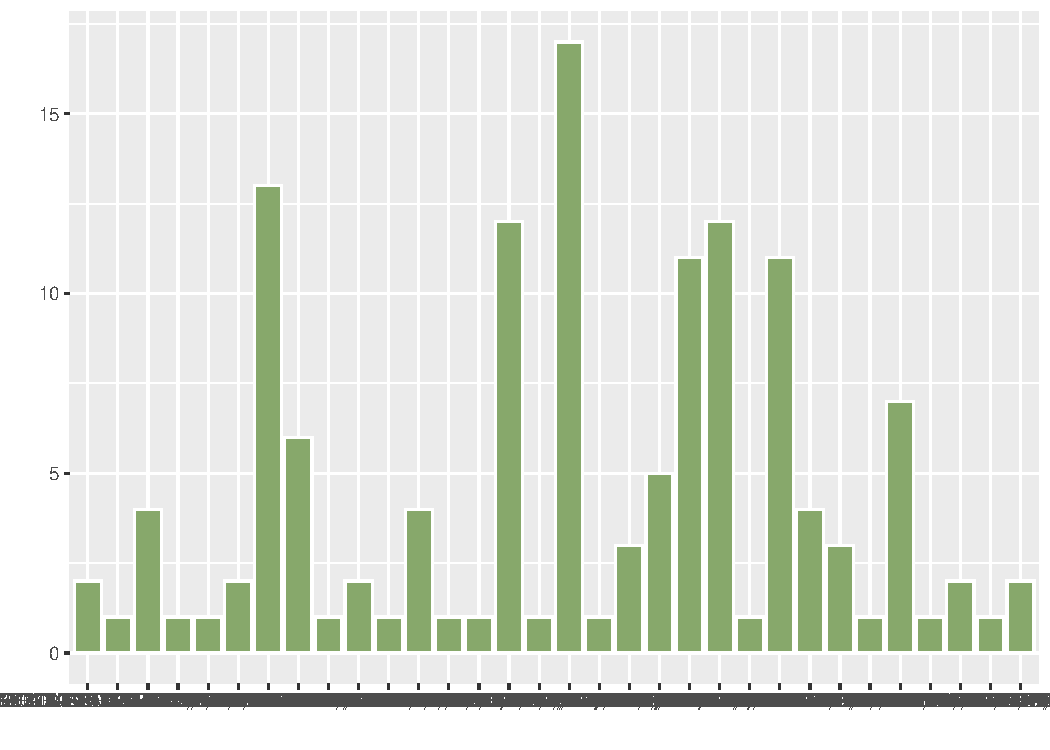
\includegraphics[width=\maxwidth]{figure/fig_treintaysiete-1} 
\end{knitrout}
}
\end{graficas}

\begin{fotos}
{trabajo de campo}{35}
\end{fotos}

\end{comment}

\begin{tablas}
{Donde realiza la comercializacion de su cosecha}{

\begin{tabular}{lcl}
\toprule
\cellcolor[HTML]{87A96B}{\textcolor{black}{\textbf{Lugar}}} & \cellcolor[HTML]{87A96B}{\textcolor{black}{\textbf{Conteo}}} & \cellcolor[HTML]{87A96B}{\textcolor{black}{\textbf{Porcentaje}}}\\
\midrule
EN MERCADOS LOCALES & 191 & 67.73\\
FERIAS AGROPECUARIAS & 16 & 5.67\\
OTRO & 6 & 2.13\\
VENTA EN LA PARCELA (CHACRA) & 40 & 14.18\\
VENTAS EN MERCADOS REGIONALES & 29 & 10.28\\
\bottomrule
\end{tabular}


}
\end{tablas}

\begin{graficas}
{Donde realiza la comercializacion de su cosecha}{
\begin{knitrout}
\definecolor{shadecolor}{rgb}{0.969, 0.969, 0.969}\color{fgcolor}
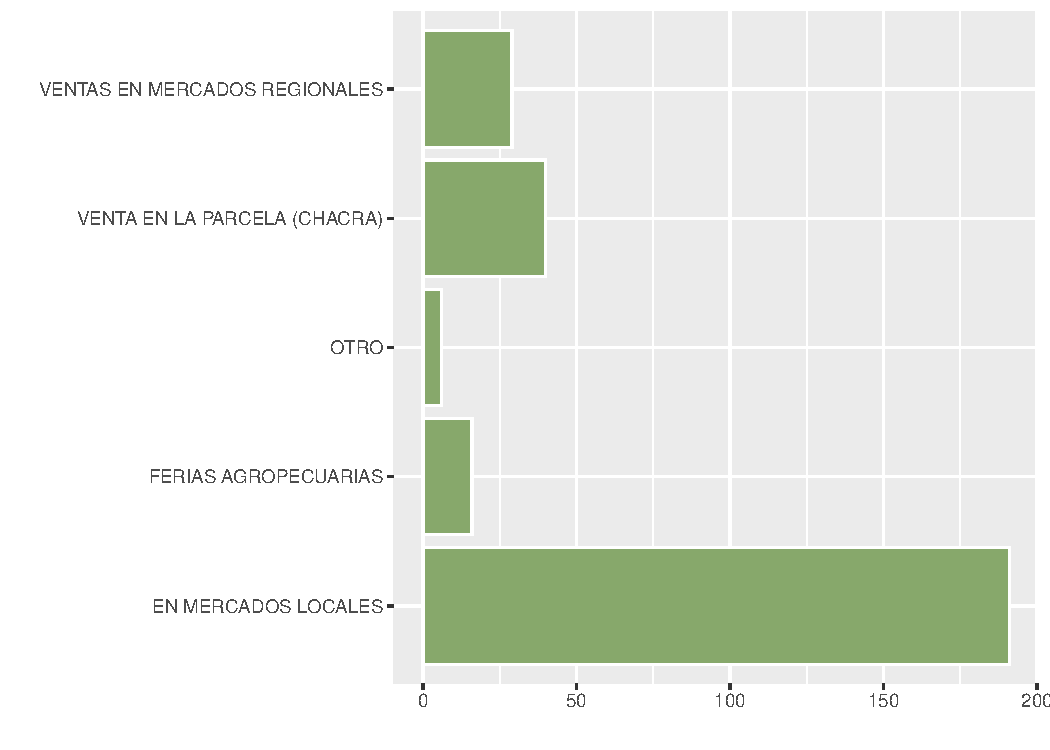
\includegraphics[width=\maxwidth]{figure/fig_treintayocho-1} 
\end{knitrout}
}
\end{graficas}

\begin{fotos}
{trabajo de campo}{36}
\end{fotos}


\begin{tablas}
{Pertenece a alguna organizacion o asociacion}{

\begin{tabular}{lcl}
\toprule
\cellcolor[HTML]{87A96B}{\textcolor{black}{\textbf{Pertenece}}} & \cellcolor[HTML]{87A96B}{\textcolor{black}{\textbf{Conteo}}} & \cellcolor[HTML]{87A96B}{\textcolor{black}{\textbf{Porcentaje}}}\\
\midrule
NO & 273 & 68.77\\
SI & 124 & 31.23\\
\bottomrule
\end{tabular}


}
\end{tablas}

\begin{graficas}
{Pertenece a alguna organizacion o asociacion}{
\begin{knitrout}
\definecolor{shadecolor}{rgb}{0.969, 0.969, 0.969}\color{fgcolor}
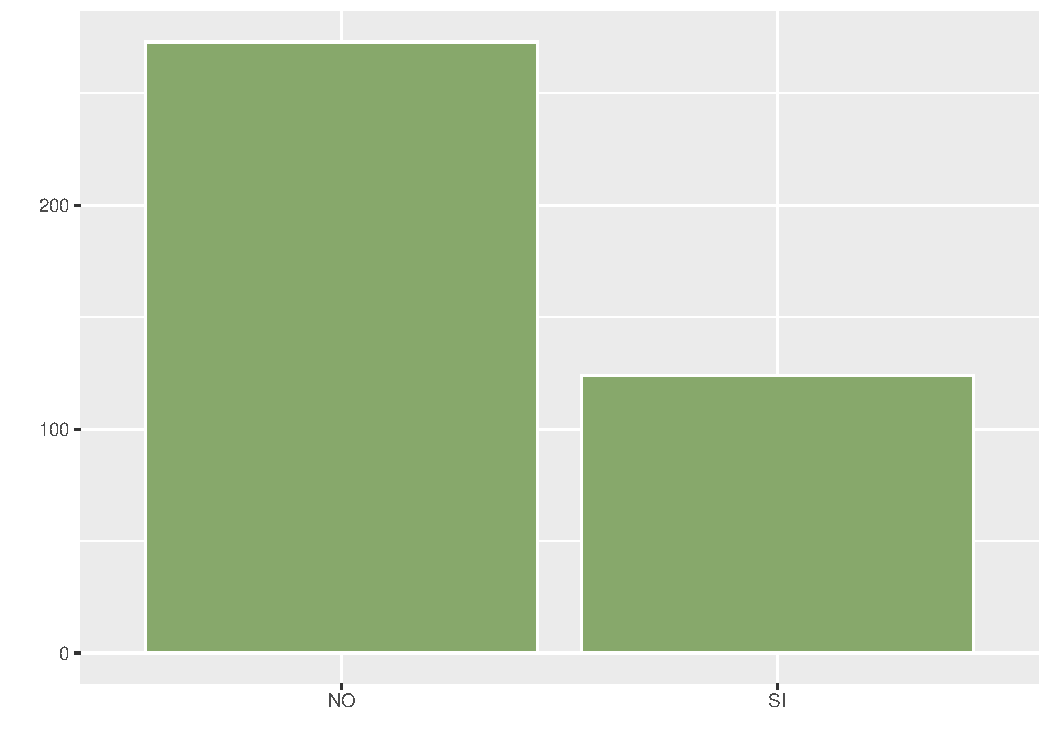
\includegraphics[width=\maxwidth]{figure/fig_treintaynueve-1} 
\end{knitrout}
}
\end{graficas}

\begin{fotos}
{trabajo de campo}{37}
\end{fotos}

\begin{comment}

\begin{tablas}
{Meses en los que realiza la cosecha}{

\begin{tabular}{lcl}
\toprule
\cellcolor[HTML]{87A96B}{\textcolor{black}{\textbf{Meses}}} & \cellcolor[HTML]{87A96B}{\textcolor{black}{\textbf{Conteo}}} & \cellcolor[HTML]{87A96B}{\textcolor{black}{\textbf{Porcentaje}}}\\
\midrule
ABRIL & 15 & 3.53\\
ABRIL, AGOSTO, DICIEMBRE & 2 & 0.47\\
ABRIL, DICIEMBRE & 1 & 0.24\\
ABRIL, MAYO & 18 & 4.24\\
ABRIL, MAYO, JUNIO & 12 & 2.82\\
\addlinespace
ABRIL, MAYO, JUNIO, JULIO & 1 & 0.24\\
ABRIL, MAYO, JUNIO, JULIO, AGOSTO, SETIEMBRE & 1 & 0.24\\
AGOSTO & 2 & 0.47\\
ENERO, ABRIL, MAYO, SETIEMBRE & 1 & 0.24\\
ENERO, AGOSTO, DICIEMBRE & 1 & 0.24\\
\addlinespace
ENERO, DICIEMBRE & 1 & 0.24\\
ENERO, FEBRERO, MARZO & 1 & 0.24\\
ENERO, FEBRERO, MARZO, ABRIL & 1 & 0.24\\
ENERO, FEBRERO, MARZO, ABRIL, MAYO & 1 & 0.24\\
ENERO, FEBRERO, MARZO, ABRIL, MAYO, JUNIO & 5 & 1.18\\
\addlinespace
ENERO, FEBRERO, MARZO, ABRIL, MAYO, JUNIO, JULIO & 10 & 2.35\\
ENERO, FEBRERO, MARZO, ABRIL, MAYO, JUNIO, JULIO, AGOSTO & 2 & 0.47\\
ENERO, FEBRERO, MARZO, ABRIL, MAYO, JUNIO, JULIO, AGOSTO, SETIEMBRE, OCTUBRE, DICIEMBRE & 35 & 8.24\\
ENERO, FEBRERO, MARZO, MAYO, AGOSTO, DICIEMBRE & 1 & 0.24\\
ENERO, FEBRERO, MARZO, MAYO, JUNIO & 1 & 0.24\\
\addlinespace
ENERO, FEBRERO, MARZO, MAYO, JUNIO, JULIO & 3 & 0.71\\
ENERO, FEBRERO, MAYO & 1 & 0.24\\
ENERO, FEBRERO, MAYO, JUNIO, JULIO & 2 & 0.47\\
ENERO, FEBRERO, MAYO, JUNIO, JULIO, DICIEMBRE & 1 & 0.24\\
ENERO, MAYO, DICIEMBRE & 2 & 0.47\\
\addlinespace
FEBRERO & 5 & 1.18\\
FEBRERO, MARZO & 4 & 0.94\\
FEBRERO, MARZO, ABRIL & 1 & 0.24\\
FEBRERO, MARZO, MAYO, JUNIO & 1 & 0.24\\
FEBRERO, MAYO & 2 & 0.47\\
\addlinespace
JULIO & 3 & 0.71\\
JULIO, AGOSTO & 1 & 0.24\\
JUNIO & 57 & 13.41\\
JUNIO, DICIEMBRE & 2 & 0.47\\
JUNIO, JULIO & 19 & 4.47\\
\addlinespace
JUNIO, JULIO, AGOSTO & 3 & 0.71\\
MARZO & 1 & 0.24\\
MARZO, ABRIL & 4 & 0.94\\
MARZO, ABRIL, MAYO & 1 & 0.24\\
MARZO, ABRIL, MAYO, JUNIO & 2 & 0.47\\
\addlinespace
MARZO, ABRIL, MAYO, JUNIO, JULIO & 1 & 0.24\\
MARZO, JULIO, OCTUBRE & 1 & 0.24\\
MARZO, JUNIO & 1 & 0.24\\
MARZO, JUNIO, JULIO & 1 & 0.24\\
MARZO, MAYO, JULIO, SETIEMBRE & 1 & 0.24\\
\addlinespace
MARZO, MAYO, JUNIO, JULIO, DICIEMBRE & 1 & 0.24\\
MARZO, MAYO, OCTUBRE & 1 & 0.24\\
MAYO & 93 & 21.88\\
MAYO, JULIO & 2 & 0.47\\
MAYO, JUNIO & 81 & 19.06\\
\addlinespace
MAYO, JUNIO, AGOSTO, OCTUBRE & 1 & 0.24\\
MAYO, JUNIO, DICIEMBRE & 1 & 0.24\\
MAYO, JUNIO, JULIO & 9 & 2.12\\
MAYO, JUNIO, JULIO, AGOSTO & 3 & 0.71\\
OCTUBRE & 1 & 0.24\\
\bottomrule
\end{tabular}


}
\end{tablas}

\begin{graficas}
{Meses en los que realiza la cosecha}{
\begin{knitrout}
\definecolor{shadecolor}{rgb}{0.969, 0.969, 0.969}\color{fgcolor}
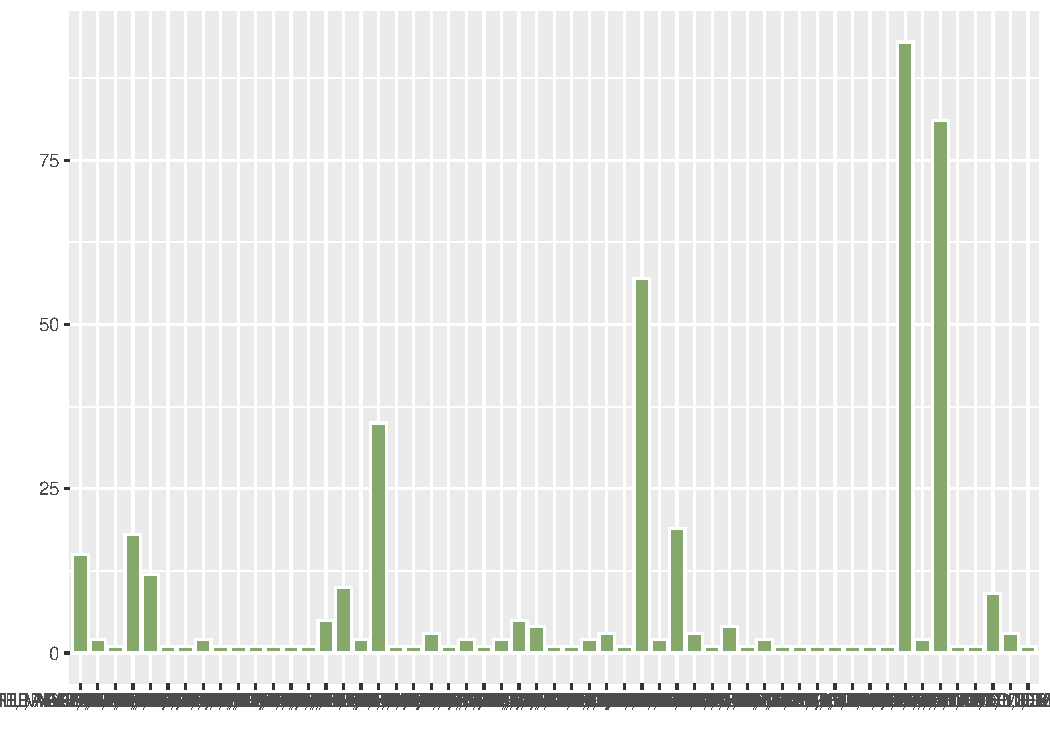
\includegraphics[width=\maxwidth]{figure/fig_cuarenta-1} 
\end{knitrout}
}
\end{graficas}

\begin{fotos}
{trabajo de campo}{38}
\end{fotos}

\end{comment}

\begin{tablas}
{Insumos que usa para la produccion y cosecha}{

\begin{tabular}{lcl}
\toprule
\cellcolor[HTML]{87A96B}{\textcolor{black}{\textbf{Insumo}}} & \cellcolor[HTML]{87A96B}{\textcolor{black}{\textbf{Conteo}}} & \cellcolor[HTML]{87A96B}{\textcolor{black}{\textbf{Porcentaje}}}\\
\midrule
ANIMALES Y HERRAMIENTAS & 105 & 26.05\\
ANIMALES Y MAQUINARIA AGRICOLA & 3 & 0.74\\
HERRAMIENTAS MANUALES & 59 & 14.64\\
HERRAMIENTAS Y MAQUINARIA AGRICOLA & 113 & 28.04\\
HERRAMIENTAS, ANIMALES Y MAQUINARIA AGRICOLA & 96 & 23.82\\
\addlinespace
IMPLEMENTOS TIRADO POR ANIMALES & 3 & 0.74\\
MAQUINARIA AGRICOLA & 24 & 5.96\\
\bottomrule
\end{tabular}


}
\end{tablas}

\begin{graficas}
{Insumos que usa para la produccion y cosecha}{
\begin{knitrout}
\definecolor{shadecolor}{rgb}{0.969, 0.969, 0.969}\color{fgcolor}
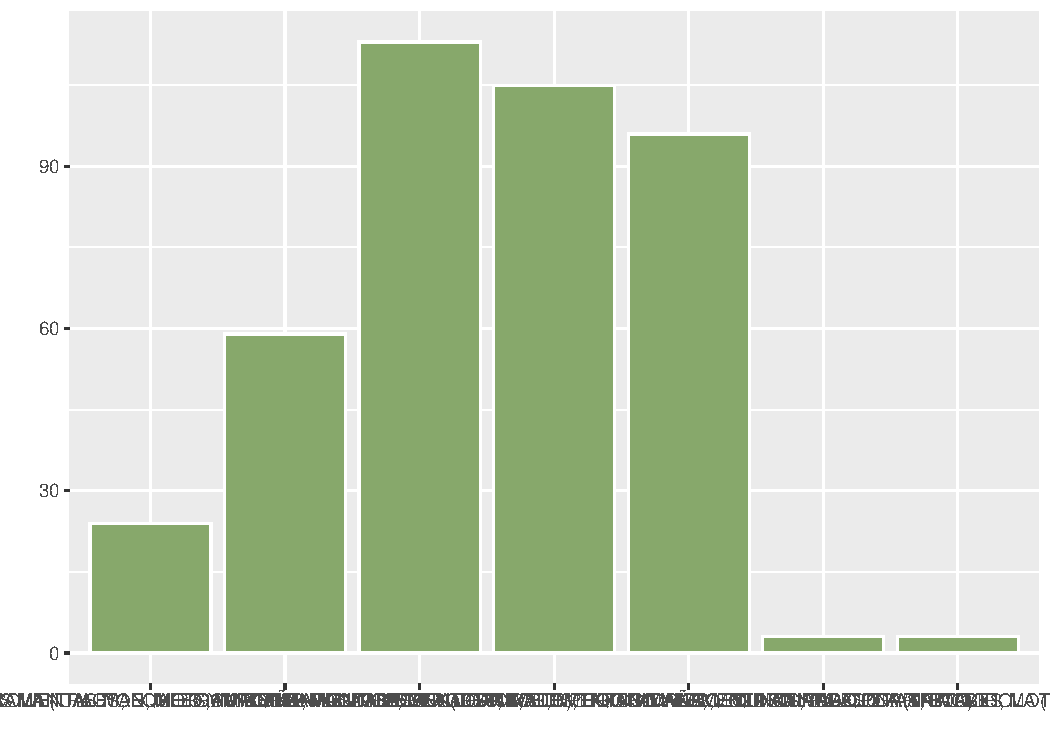
\includegraphics[width=\maxwidth]{figure/fig_cuarentayuno-1} 
\end{knitrout}
}
\end{graficas}

\begin{fotos}
{trabajo de campo}{39}
\end{fotos}

%para hacer commit desde la terminal:
%git add .
%git commit -m "Actualizacion de archivos (esto se puede modificar) .Rnw"
%para hacer push
%git push origin main

%para crear una nueva rama en la terminal
%git branch Marina
%para cambiar a la nueva rama 
%git checkout Marina
%para subir la nueva rama a github
%git push -u origin Marina

cambio desde main
\end{document}
